\chapter{Learning Stable Periodic Robot Motions from Demonstration}
\label{chp:osmp}

\begin{foreword}
    % So far, this thesis has focused mostly on the application of (learned) models within shape sensing and control. Yet, when working towards fully autonomous robots, one of the most challenging research topics is high-level decision making as the controllers that we have considered in this thesis all need either a setpoint or a trajectory to track. In Chapter~\ref{chp:braincontrol}, we introduced an approach to how users could directly control the robot with their thoughts by moving setpoints in space. However, while such low-level \gls{HRI} allows the human to control the robot's actions with vast detail, this requires the full attention of the user and is exhausting for the user, reducing some of the potential efficiency improvements that we envision robots to allow for. A promising alternative could be that the user communicates only high-level tasks to the robot, and the robot plans its motion by itself. Apart from \gls{RL} or optimization-based motion planning strategies such as \gls{MPC}, one of the most promising avenues here is \glsxtrfull{LFD}. Specifically, for 20 years, there has already been literature on learning motion policies with dynamical systems~\citep{ijspeert2013dynamical}, which the community refers to as \glsxtrfull{DMP}. In recent years, the advent of deep learning and normalizing flows~\citep{kobyzev2020normalizing} introduced the new concept of \glsxtrfull{SMP}, where a diffeomorphic mapping into latent space parametrized by a neural network is combined with a latent dynamical system~\citep{rana2020euclideanizing, perez2023stable, zhi2024teaching}. This allows the learning of more complex behaviors while preserving interpretability and stability guarantees. In this chapter, we extend the framework of \gls{SMP} to learning periodic motions while guaranteeing the orbital stability of the system.  We achieve this by combining a bijective encoder based on Euclideanizing flows with latent dynamics based on the supercritical Hopf bifurcation. This concept shares as similar spirit as in Chapter~\ref{chp:con}, although we now apply it to motion policies instead of learned dynamical models.
    % improved version by ChatGPT
    This thesis has so far concentrated primarily on the use of learned models in shape sensing and control. However, a critical challenge in achieving fully autonomous robots lies in high-level decision-making. The controllers discussed in this work require either a setpoint or a trajectory to follow. In Chapter~\ref{chp:braincontrol}, we explored a method enabling users to guide the soft robot directly through their thoughts by manipulating setpoints in space, which a compliant impedance controller subsequently tracks. While this low-level \gls{HRI} provides precise control over the robot’s actions, it demands the user’s full attention and can become exhausting, thereby limiting the efficiency gains we expect to gain by introducing intelligent, autonomous robots.
    %
    An alternative approach involves the user specifying only high-level tasks, allowing the robot to plan its motions independently. Among potential methods, including \gls{RL} and optimization-based strategies like \gls{MPC}, \gls{LFD} stands out as particularly promising as it allows the learning of complex motions from humans or even from other biological creatures. As a special case of \gls{LFD}, research on learning motion policies using dynamical systems has been well-established~\citep {ijspeert2013dynamical}. Being referred to as \glsxtrfull{DMP} or \glsxtrfull{SMP}, this strategy exhibits interpretability, compliant behavior, and convergence guarantees. Recently, advances in deep learning and normalizing flows~\citep{kobyzev2020normalizing} have given rise to frameworks that increase the expressiveness of the motion policy by leveraging diffeomorphic mappings into latent spaces, parametrized by neural networks, combined with latent dynamical systems~\citep{rana2020euclideanizing, perez2023stable, zhi2024teaching}. These methods enable the learning of more complex behaviors while maintaining interpretability, stability, and convergence guarantees.
    %
    In this chapter, we extend this approach to learn periodic motions with guaranteed orbital stability. This is achieved by integrating a bijective encoder based on Euclideanizing flows with latent dynamics modeled as supercritical Hopf bifurcations. The approach aligns in terms of vision with the work in Chapter~\ref{chp:con}, but here, it is applied to motion policy rather than dynamical model learning.
\end{foreword}

\pagebreak

\begin{abstract}
    % As we strive for humans and robots to collaborate closely or to have robots assist us in tasks of daily living, we need to make sure that the robots exhibit compliant, natural, and predictable behavior. 
    % Motion primitives represent velocity (or acceleration) fields that allow us to encode motions without any explicit time dependence and exhibit natural and compliant behaviors even under significant perturbations.
    % In recent years, there has been a strong push to leverage linear latent dynamics with a learned bijective encoder for learning stable, point-to-point motion primitives from demonstrations. However, existing approaches are not able to encode periodic motions.
    % In this work, we present how supercritical Hopf bifurcations in latent space allow for learning periodic motions from demonstration with stability guarantees. We introduce additional techniques such as phase synchronization, latent velocity shaping, and encoder conditioning that allow us to tackle complex, periodic robotic tasks such as turtle swimming or surface cleaning.
    % This will allow collaborative robots to perform periodic motions in an accurate, compliant, stable, and natural fashion and, with that, bring us one step closer to safe and intuitive human-robot collaboration.
    As we aim to foster closer collaboration between humans and robots—or to have robots assist us in everyday tasks—it is essential that these machines exhibit behavior that is robust, compliant, and natural. 
    Learning from demonstrations has proven to be a powerful approach for acquiring complex motion behaviors in a sample-efficient manner compared to methods like reinforcement learning.
    However, many current techniques—such as state-of-the-art diffusion policies—still require a large number of demonstrations to cover most state-action pairs, as these models lack inherent convergence guarantees.
    In contrast, dynamic motion primitives, which parameterize motion policies using dynamical systems, provide such convergence guarantees—often referred to as stable motion primitives—while maintaining natural and compliant behavior even under significant disturbances.
    Recent efforts have focused on leveraging linear latent dynamics paired with a learned, bijective encoder to derive stable, point-to-point motion primitives from demonstrations. However, these methods have fallen short when it comes to encoding periodic motions. In this work, we demonstrate that employing supercritical Hopf bifurcations in latent space can effectively learn periodic motions from demonstrations while ensuring stability. We further introduce techniques such as phase synchronization, online shaping of the convergence behavior, and encoder conditioning, which empower us to address complex periodic robotic tasks like turtle swimming and surface cleaning. These advancements pave the way for collaborative robots to perform periodic motions accurately, compliantly, stably, and naturally—bringing us one step closer to safe and intuitive human-robot interaction.
\end{abstract}

\blfootnote{This chapter is partly based on \faFileTextO ~\emph{\textbf{M. Stölzle}, T.K. Rusch*, Z.J. Patterson*, R. Pérez Dattari, F. Stella, J. Hughes, C. Della Santina, and D. Rus (2025). Learning Stable Periodic Robotic Motions from Demonstration. % In Science Robotics, 
\textbf{\emph{In Preparation}}}.
}

%% Start the actual chapter on a new page.
\newpage

\section{Introduction}
\dropcap{I}mitation Learning \citep{schaal1999imitation, zare2024survey} has regained substantial traction in recent years due to its superior sample and iteration efficiency in acquiring complex tasks compared to Reinforcement Learning. Recent work has focused on improving the robustness, expressiveness, and generalization of motion policies learned from demonstration by leveraging modern ML architectures such as diffusion models and flow matching~\citep{chi2023diffusion, black2024pi0}; scaling up the number of demonstrations to increase robustness~\citep{o2024open, black2024pi0, gemini2025robotics}; training across multiple robot embodiments (e.g., different manipulators) to promote generalization~\citep{o2024open, black2024pi0}; and conditioning policies on semantic task instructions and environment context via embeddings from large \glspl{VLM}~\citep{black2024pi0, gemini2025robotics}.
Among these, \glspl{DMP}~\citep{ijspeert2002learning, ijspeert2013dynamical, saveriano2023dynamic, hu2024fusion} parametrize a motion policy through dynamical systems that predict the desired velocity or acceleration based on the system’s current state. By grounding the formulation in dynamical systems, researchers can leverage established tools from nonlinear system theory~\citep{khalil2002nonlinear} to analyze and ensure-by-design convergence properties in motion primitive—such as global asymptotic stability~\citep{kober2009learning, ijspeert2013dynamical, rana2020euclideanizing, urain2020imitationflow, zhang2022learning, perez2023stable, perez2024puma} or orbital stability~\citep{ijspeert2002learning, kober2009learning, wensing2017sparse, urain2020imitationflow, khadivar2021learning, abu2021periodic, abu2024learning, zhi2024teaching, nah2025combining}. This is not typically the case for other ML-based motion policies like RNNs or Diffusion Policies (DPs)~\citep{chi2023diffusion, o2024open, black2024pi0, gemini2025robotics}.
Such approaches—often referred to as \glspl{SMP}—are robust to perturbations, disturbances, and model mismatches, as the motion policy continuously steers the system back to the desired reference. This also enhances data efficiency, a trait that is increasingly important as robots take on a broader range of tasks.

An important subclass of \gls{DMP} strategies addresses tasks that require continuous, non-resting motion—those for which rest-to-rest trajectories are neither representative nor sufficient. Canonical examples include wiping a surface, swimming, or walking, where motion generation must produce sustained activity across cycles. These so-called rhythmic or periodic \glspl{DMP} have spurred extensive research, both within the traditional dynamical systems formulation~\citep{ijspeert2002learning,kober2009learning,ijspeert2013dynamical,wensing2017sparse,kramberger2018passivity,saveriano2023dynamic,abu2024learning,hu2024fusion,nah2025combining} and in more recent methods combining simple latent-space limit cycles with learned diffeomorphic mappings~\citep{urain2020imitationflow,khadivar2021learning,zhi2024teaching}. Still, despite these advances, existing approaches struggle to reproduce non-trivial trajectories—especially those with sharp transitions, high curvature, or discontinuous velocity profiles, which are common in real-world rhythmic tasks. Overcoming this typically requires many demonstrations, thus strongly limiting their applicability in practical settings. 

Such limitations are exacerbated by the incapability of classical deterministic \glspl{DMP} to generalize across tasks~\citep{jaquier2025transfer}: a fresh or fine-tuned model must be trained for every new motion or task \citep{saveriano2023dynamic}. Although several studies have introduced task-conditioned variants—such as conditioning on encoded visual observations~\citep{bahl2020neural, mohammadi2024extended} or adopting probabilistic \glspl{DMP} formulations~\citep{seker2019conditional, saveriano2023dynamic, pekmezci2024coupled}—these methods often yield incoherent trajectories when presented with tasks they did not explicitly encounter during training~\citep{jaquier2025transfer}, even when those tasks lie within the original training distribution. 

So, despite their promise of being an alternative to data-intensive learning strategies, \glspl{DMP} ultimately require a substantial amount of data and a complex training process when tasks are varied and trajectories are not straightforward. Instead, the ability to generate purposeful motions in zero-shot settings for unseen tasks will be essential on the path towards truly generalist autonomous robots in the future.

In this paper, we introduce \glspl{OSMP}, a framework, visualized in Fig.~\ref{fig:osmp:concept_overview}, designed to address the limitations of existing rhythmic motion primitives by learning an expressive, orbitally stable limit cycle capable of capturing elaborate periodic behaviors. Our approach imposes a dynamic inductive bias by shaping the latent space according to a supercritical Hopf bifurcation oscillator; a well-studied system in nonlinear dynamics~\citep{strogatz2018nonlinear, khadivar2021learning, nah2025combining} that has remained unexplored in the context of machine learning. This core dynamical prior is complemented by a novel bijective Euclideanizing-flow encoder, extending the Real NVP architecture~\citep{rana2020euclideanizing, dinh2017density}.

Under mild architectural assumptions, we prove \glspl{OSMP} are almost-globally transverse contracting, so every trajectory converges exponentially—not merely asymptotically—to the learned limit cycle. A tailored loss suite binds the cycle’s shape and speed to the demonstration, eliminating the long-standing mismatch between a stable latent orbit and a highly curved, nonlinear sample. Thus, a single demonstration already yields an effective policy, drastically outperforming the data efficiency of DPs~\citep{chi2023diffusion}. 
A novel conditioning–interpolation loss then drives smooth, zero-shot transitions between related tasks: for example, the model continuously morphs between reverse and forward turtle-swimming gaits after seeing only those two exemplars. This ability sharply reduces the need to densely sample the motion task space and further increases data efficiency. 
We also introduce solutions for synchronizing multiple primitives in their phase and, without retraining, affinely scale, translate, or otherwise modulate the learned velocity field, turning rhythmic \glspl{DMP} into a practical, data-efficient controller for complex robots.

We rigorously validate our approach in both simulation and on hardware. Quantitative and qualitative benchmarks compare it with classical neural models (\glspl{MLP}, \glspl{RNN}, \glspl{NODE}), state-of-the-art motion policies like \gls{DP}~\citep{chi2023diffusion}, and diffeomorphic-encoder methods with stable latent dynamics, including Imitation Flow (iFlow)~\citep{urain2020imitationflow} and \gls{SPDT}~\citep{zhi2024teaching}. Experiments show our \glspl{OSMP} accurately track periodic trajectories on diverse robotic platforms—UR5 and Kuka arms, the Helix soft robot, and a hybrid underwater “crush turtle” robot. Expressed as autonomous dynamical systems, they deliver more compliant, natural behavior than time-indexed, error-based controllers. We further demonstrate in both simulations and real-world experiments in-phase synchronization of multiple \glspl{OSMP} and, via encoder conditioning, smooth interpolation among several distinct motion tasks with a single motion policy.

\begin{figure}[h!]
    \centering
    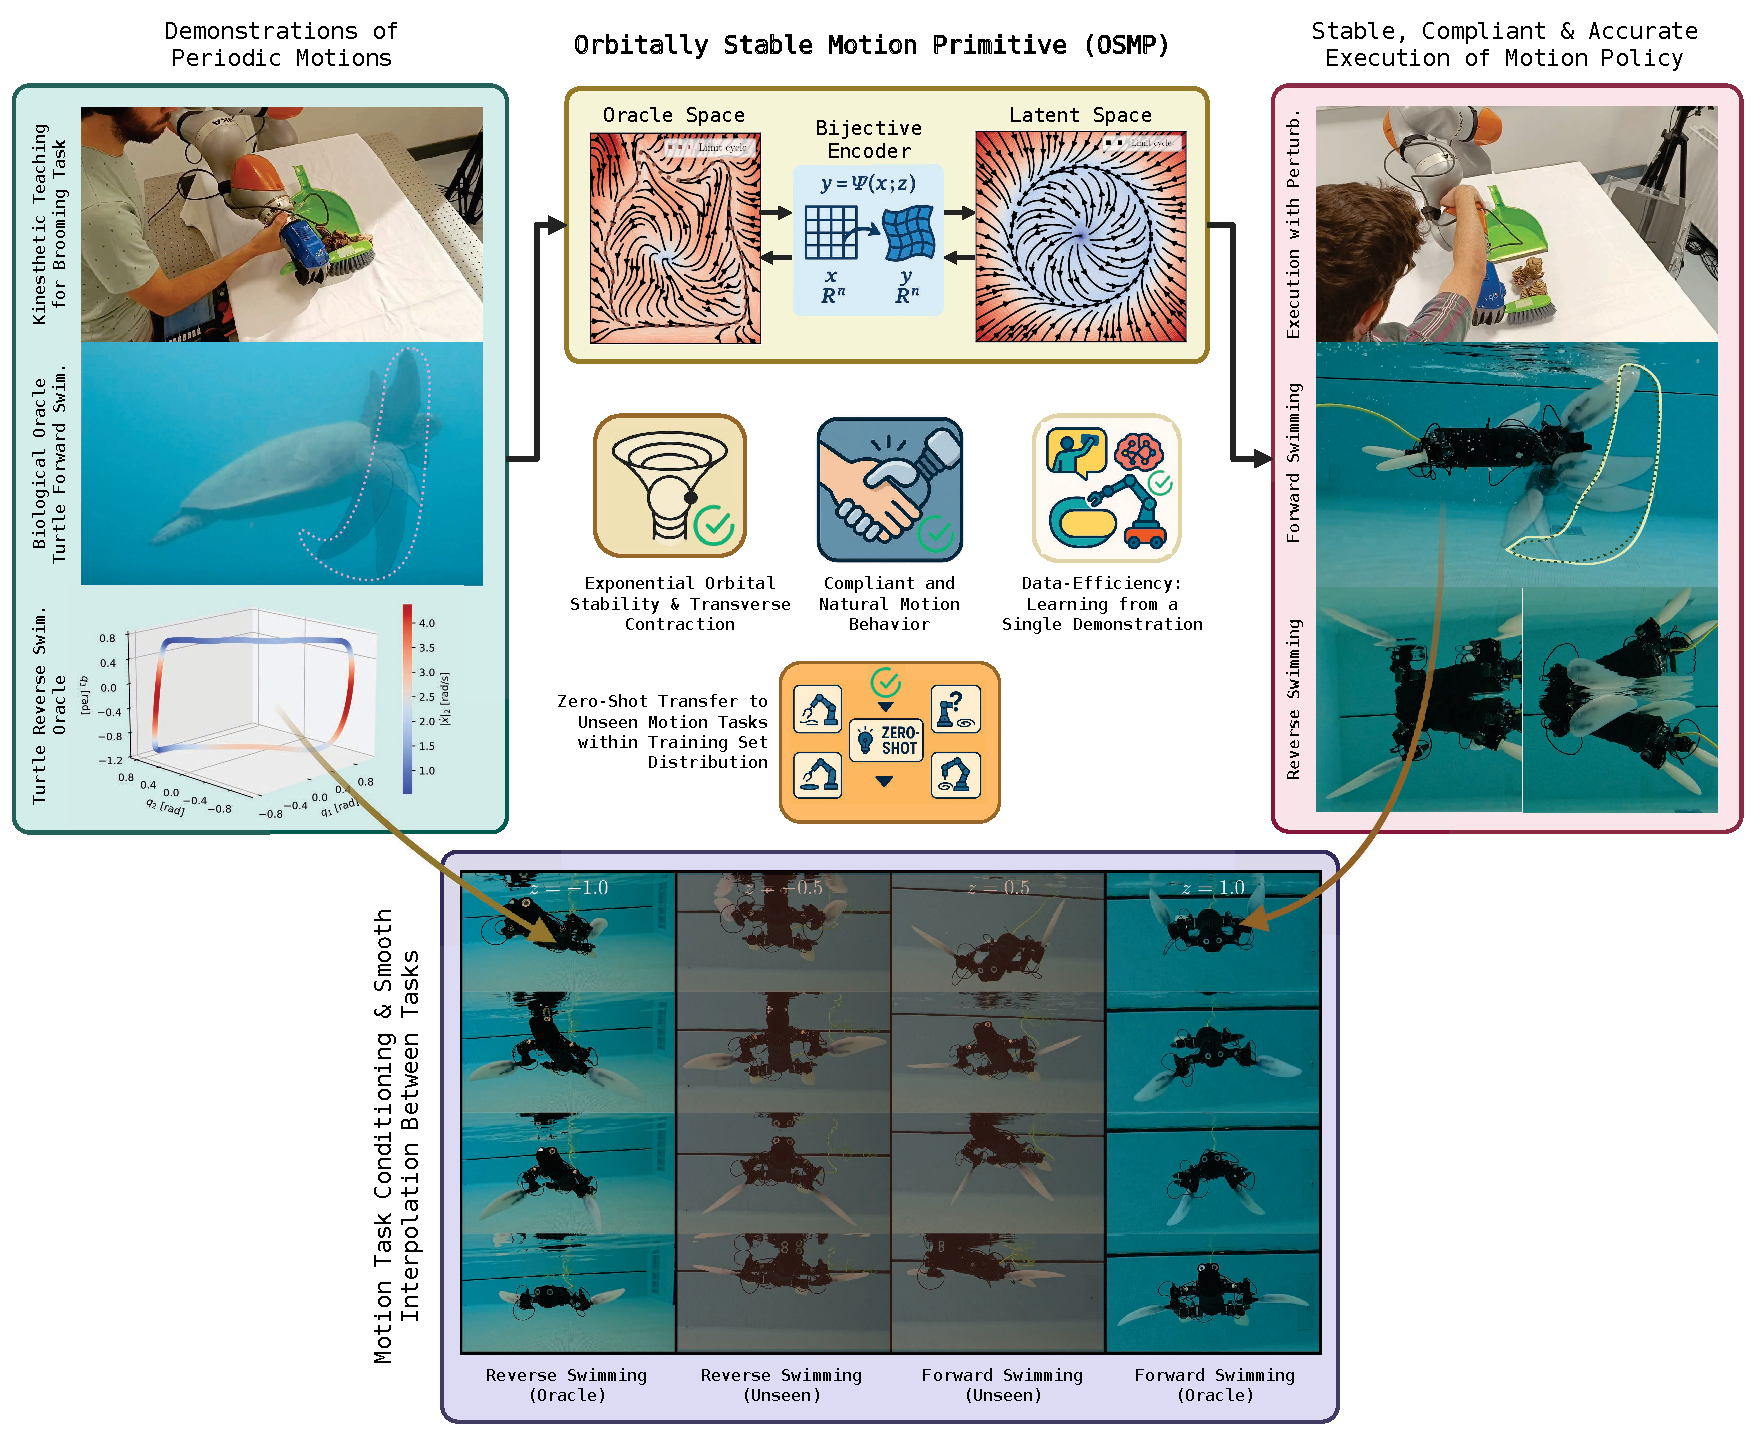
\includegraphics[width=1.0\linewidth]{osmp/figures/concept_overview/concept_overview_v1_compressed.pdf}
    % \includesvg[width=1.0\linewidth]{figures/methodology_overview/osmp_methodology_overview_v2.svg}
    \caption{
    \textbf{Overview of Features and Characteristics of \glspl{OSMP}.}
    OSMPs enable the learning of periodic motions from demonstrations while guaranteeing exponential orbital stability \& transverse contraction, instilling compliant and natural motion behavior, and outstanding data efficiency as they are able to learn complex motion behaviors from just one demonstration. Furthermore, a motion task conditioning allows the same motion policy to exhibit multiple distinct behaviors while a specially crafted loss term encourages smooth interpolation between motion tasks seen during training leading to meaningful motion behaviors on task unseen during training (i.e., zero-shot transfer).
    }
    \label{fig:osmp:concept_overview}
\end{figure}


\subsection{Methodology in a Nutshell}
Below, we provide a brief overview of the \gls{OSMP} methodology and architecture, as depicted in Fig.\ref{fig:osmp:methodology_overview}. Further details are provided in Sec.~\ref{sec:osmp:methodology}. In the \gls{DMP} framework, an \gls{OSMP} outputs the desired system velocity as $\dot{x}=f(x; z)$, with $x\in\mathbb{R}^n$ the configuration and $z$ the motion-task conditioning. The computation proceeds in three steps: (i) map $x$ into a latent coordinate $y\in\mathbb{R}^n$ using a $z$-conditioned bijective encoder (a learned diffeomorphism); (ii) evaluate the designed latent dynamics to obtain $\dot{y}$; and (iii) project $\dot{y}$ back to the original space via the encoder’s inverse Jacobian. While the architecture can be trained under various regimes (e.g., reinforcement learning), this paper focuses on imitation learning—specifically, behavior cloning—where both the latent representation y and the predicted velocity $\dot{x}$ are supervised.

\subsection{Related Work}
While there is a long history of research on both discrete and rhythmic/periodic \glspl{DMP}~\citep{ijspeert2002learning, kober2009learning, ijspeert2013dynamical, wensing2017sparse, kramberger2018passivity, saveriano2023dynamic, abu2024learning, hu2024fusion, nah2025combining}, the expressive power of classical \glspl{DMP}~\citep{ijspeert2002learning, kober2009learning, ijspeert2013dynamical, wensing2017sparse} is limited, preventing them from learning highly complex and intricate trajectories.

Recently, however, an exciting research direction has emerged that combines diffeomorphisms into a latent space—learned using ML techniques—with relatively simple, analytically tractable (e.g., linear) latent space dynamics to enhance expressiveness while preserving stability and convergence guarantees~\citep{rana2020euclideanizing, urain2020imitationflow, zhang2022learning, perez2023stable}. Most of these works focus on point-to-point motions and aim to ensure global asymptotic stability~\citep{rana2020euclideanizing, zhang2022learning, perez2023stable, perez2024puma}, although there have also been several works combining diffeomorphic encoders with rhythmic latent dynamics for learning periodic motions from demonstration~\citep{urain2020imitationflow, khadivar2021learning, zhi2024teaching}.
However, in the existing methods, either the chosen architecture for the bijective encoder lacks expressiveness~\citep{urain2020imitationflow, khadivar2021learning}, the method training is very sensitive to the initial neural network parameter~\citep{urain2020imitationflow}, the method does not learn the demonstrated velocities but only the general direction of motion~\citep{zhi2024teaching}, or cannot accurately learn very complex oracle shapes~\citep{zhi2024teaching}.

Although the proposed model architecture is similar to that of \citet{zhi2024teaching}, our training pipeline differs substantially: we incorporate an imitation loss that teaches the model the demonstrated velocities, replace the Hausdorff-distance objective with a limit-cycle matching loss better suited to complex or discontinuous paths, optionally guide latent polar angles with a time-alignment term to capture highly curved, possibly concave, contours, and regularize workspace velocities outside the demonstration to improve numerical stability during inference. 
Finally, we allow a parametrization of the polar angular velocity with a neural network, allowing the learning of complex velocity profiles along the limit cycle without compromising the strong contraction guarantees. 

Furthermore, the above-mentioned methods do not offer solutions for many practical issues, such as synchronizing multiple systems—a common requirement in locomotion or bimanual manipulation~\citep{gams2015accelerating}—or to shape the learned velocity online.

We provide a comparison with relevant existing methods in Table~\ref{tab:osmp:osmp_characteristics_vs_baselines}.

\begin{figure}[h!]
    \centering
    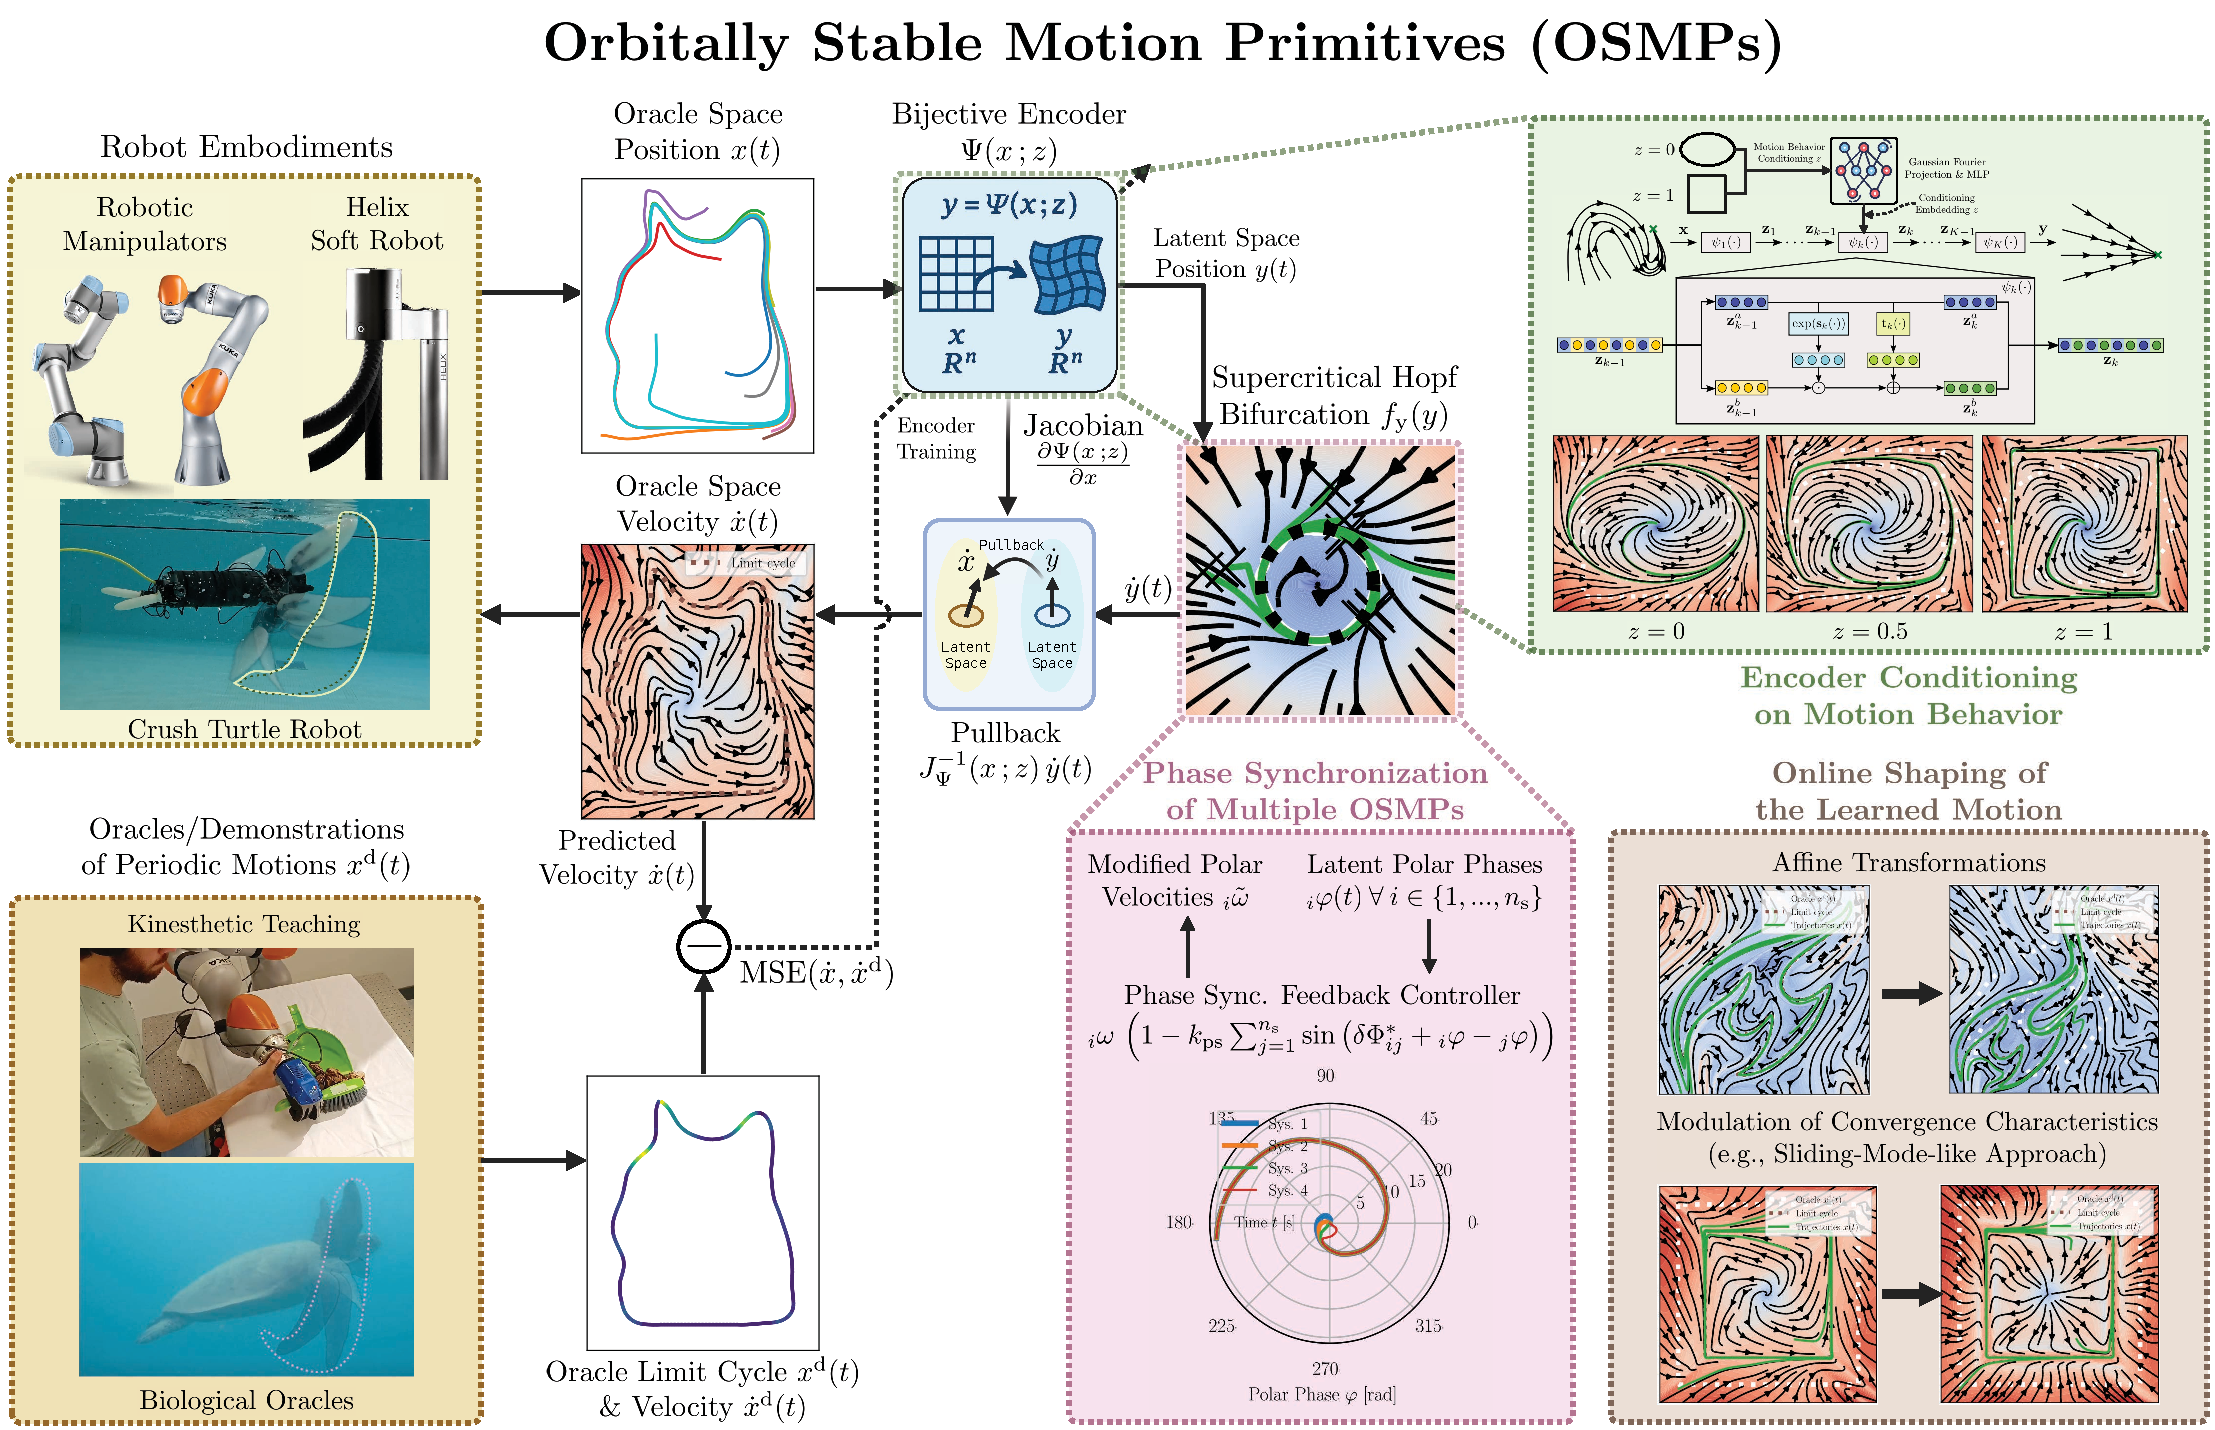
\includegraphics[width=1.0\linewidth]{osmp/figures/methodology_overview/osmp_methodology_overview_v3_compressed.pdf}
    % \includesvg[width=1.0\linewidth]{figures/methodology_overview/osmp_methodology_overview_v2.svg}
    \caption{
    \textbf{Methodology of \glspl{OSMP}.}
    Periodic motions can be learned from demonstration via a \gls{DMP} that combines a bijective encoder with latent space dynamics defined by a supercritical Hopf bifurcation. After encoding the current oracle space position of the system into latent space and predicting the latent space velocity, the pullback operator projects the velocity back into oracle space and represents a motion reference for the various robot embodiments. During training, we enforce both the predicted velocity and the exhibited limit cycle to match the demonstrations that are, for example, provided via kinesthetic teaching or based on biological oracles.
    Multiple contributions increase the practical usefulness of the proposed methods, which include a technique to synchronize multiple \glspl{OSMP} in phase, an approach to shape the learned motion online without requiring retraining via affine transformations or even modulating the convergence characteristics, and a methodology for conditioning the encoder on the oracle which allows the \gls{OSMP} to capture multiple distinct motion behaviors and even smoothly interpolate between them.
    The depiction of the Euclideanizing flows architecture is adapted from \citet{rana2020euclideanizing}.
    }
    \label{fig:osmp:methodology_overview}
\end{figure}

\begin{table}
    \centering
    % Captions go above tables
    \caption{\textbf{Comparison of characteristics of proposed methods against relevant baseline methods.} 
    In some cases, we denote with a \emph{x$^*$} that the feature could (probably) be developed for the respective method, but was not presented in the original paper.
    \emph{Note:} The CLF-CBF-NODE only guarantees convergence to a target trajectory as predicted by the learned NODE. However, the learned NODE is not guaranteed to exhibit a stable limit cycle behavior.
    }
    \label{tab:osmp:osmp_characteristics_vs_baselines} % give each table a logical label name
    \begin{scriptsize}
    \setlength\tabcolsep{2.0pt}
    \begin{tabular}{l ccccccc}\\
        \toprule
        \textbf{Method} & \textbf{Model} & \textbf{Orb. Stability} & \textbf{Velocity} & \textbf{$N$-Policies} & \textbf{Task} & \textbf{Smooth Task}\\
        & \textbf{Expressiveness} & \textbf{Guarantees} & \textbf{Imitation} & \textbf{Sync.} & \textbf{Conditioning} & \textbf{Interpolation}\\
        \midrule
        \gls{MLP} \& \gls{RNN} & Moderate & x & Noisy & x & $\checkmark$ & x\\
        \gls{NODE} & Moderate & x & $\checkmark$ & x & $\checkmark$ & x\\
        \gls{DP}~\citep{chi2023diffusion} & High & x & Noisy & x & $\checkmark$ & x\\
        Classical Rhythmic \glspl{DMP}  & Limited & $\checkmark$ & $\checkmark$ & $\checkmark$ & x & x\\
        HB-GMR~\citep{khadivar2021learning} & Limited & $\checkmark$ & x & x$^*$ & x & x\\
        Imitation Flow (iFlow)~\citep{urain2020imitationflow} & Moderate & $\checkmark$ &  $\checkmark$ & x$^*$ & x$^*$ & x\\
        CLF-CBF-NODE~\citep{nawaz2024learning} & Moderate & x & $\checkmark$ & x & x$^*$ & x\\
        \gls{SPDT}~\citep{zhi2024teaching} & Moderate & $\checkmark$ & x & x$^*$ & x & x\\
        \textbf{\gls{OSMP} (ours)} & Moderate & $\checkmark$ & $\checkmark$ & $\checkmark$ & $\checkmark$ & $\checkmark$\\
        \bottomrule
    \end{tabular}
    \end{scriptsize}
\end{table}
\section{Methodology}
In this work, we introduce \glspl{OSMP}, which can be trained to capture complex periodic motions from demonstrations while ensuring convergence to a limit cycle that aligns with a predefined oracle. To accomplish this, we build on previous research~\citep{rana2020euclideanizing, zhi2024teaching} that combines learned bijective encoders with a prescribed motion behavior in latent space. These latent dynamics generate velocities or accelerations that are subsequently mapped back into the oracle space via a pullback operator~\citep{zhang2022learning}—in the case of a bijective encoder, this operator is the inverse of the encoder’s Jacobian. In this formulation, the motion in latent space exhibits key convergence properties, such as \gls{GAS}~\citep{rana2020euclideanizing, perez2023stable, sochopoulos2024learning} or \gls{OS}~\citep{zhi2024teaching}, while the learned encoder provides the necessary expressiveness to capture complex motions and transfers the convergence guarantees from latent to oracle space through the established diffeomorphism.

However, compared to existing work~\citep{zhi2024teaching}, we introduce several crucial modifications that enhance both the performance and practical utility of the proposed method: (1) we develop a limit cycle matching loss to reduce the discrepancy between the learned limit cycle and the periodic oracle; (2) we design strategies to modulate the learned velocity field online without the need for retraining—for instance, to adjust the convergence behavior; (3) we establish a procedure to synchronize the phase of multiple \glspl{OSMP}; and (4) we condition the encoder on a task, enabling a single \gls{OSMP} to exhibit multiple distinct motion behaviors. Moreover, we introduce loss terms that allow the trained \gls{OSMP} to smoothly interpolate between the learned motion behaviors—something that has not been possible before.

\subsection{Orbitally Stable Motion Primitives}
In the framework of stable motion primitives~\citep{rana2020euclideanizing, perez2023stable, perez2024puma}, we aim to learn velocity field $\dot{x} = f(x)$ that maps the robot's position/state $x \in \mathbb{R}^n$ into the corresponding time derivative $\dot{x} \in \mathbb{R}^n$, where $n \in \mathbb{N}_{>1}$ denotes the Degrees of Freedom (DOF). Here, $x$ is typically defined in task space but can also be defined in other Cartesian or generalized coordinates (e.g., joint space). Therefore, we will in the following refer to these coordinates as \emph{Oracle space}.
In this work, we are specifically interested in cases where we train $f(x)$ to learn periodic motions.
To achieve this, we establish a connection between the oracle and a latent space via a diffeomorphism that is provided by an encoder $\psi: \mathbb{R}^n \to \mathbb{R}^n$, which maps positional states $x \in \mathbb{R}^n$ into the latent states $y \in \mathbb{R}^n$.
Optionally, this encoding is conditioned on a continuous variable $z \in \mathbb{R}$ as a homotopy such that $y = \psi(x;z)$.
Furthermore, we construct $\psi$ such that it is invertible and a closed-form inverse function $\psi^{-1}: y \mapsto x$ allows us to map from latent space back into oracle space.
In latent space, we apply dynamics $\dot{y} = f_\mathrm{y}(y)$ that exhibit a stable limit cycle behavior. In summary, the orbitally stable motion primitive is given as
\begin{equation}
    \dot{x} = f(x;z) = J_\psi^{-1}(x;z) \, f_\mathrm{y} \left (\psi(x;z) \right ),
\end{equation}\
where $J_\psi = \frac{\partial \psi(x;z)}{\partial x}$ defines the Jacobian of the encoder. 
As $\psi$ is bijective (w.r.t. $x$ and $y$), the motion policy is orbitally stable by construction~\citep{zhi2024teaching}.

\subsubsection{Diffeomorphic Encoder}

We consider a bijective encoder $\psi_\theta : \mathbb{R}^n \times \mathbb{R} \to \mathbb{R}^n$, which maps positional states $x \in \mathbb{R}^n$ into the latent states $y \in \mathbb{R}^n$ conditioned on $z \in \mathbb{R}$, where we assume that $n \in \mathbb{N} \geq 2$.
% Remark: In a slight abuse of phrasing, we refer to the encoder as bijective when the mapping $x \mapsto y$ is bijective. This, however, is sufficient for stability purposes.
The encoder $y = \psi_\theta(x;z)$ is parametrized by the learnable weights $\theta \in \mathbb{R}^{n_\theta}$. We omit $\theta$ in most subsequent expressions for simplicity of notation.
%
If a conditioning is used, the encoder first embeds it with a function $e_\mathrm{z}: \mathbb{R} \to \mathbb{R}^{n_\mathrm{e}}$, which provides $\Bar{z} = e_\mathrm{z}(z)$. Customarily, we choose $n_\mathrm{e} = n$ and construct $e_\mathrm{z}$ using a Gaussian Fourier projection~\citep{chi2023diffusion} into a dimensionality of $4 \, n_\mathrm{e}$ and a two-layer MLP with hidden dimension of $8 \, n_\mathrm{e}$ and a softplus nonlinearity.
% \textcolor{red}{TODO: explain Fourier projection in more detail}.
%
The encoder is composed by $n_\mathrm{b}$ blocks: $\psi = \psi_1 \circ \psi_2 \dots \psi_{n_\mathrm{b}}$, where $\psi_j: \chi_{j-1} \in \mathbb{R}^n \in \mathbb{R} \mapsto \chi_{j} \in \mathbb{R}^n$. Therefore, $\chi_0 = x$ and $\chi_{n_\mathrm{b}} = y$.
In particular, we employ Euclideanizing flows~\citep{dinh2017density, rana2020euclideanizing}, which splits $\chi_j$ into two parts: $\chi_\mathrm{a} \in \mathbb{R}^{n_\mathrm{a}}$ and $\chi_\mathrm{b} \in \mathbb{R}^{n_\mathrm{b}}$ with $n_\mathrm{a} + n_\mathrm{b} = n$.
%
Then, for odd and even $j$, $\psi_j$ is given by
\begin{equation}
    \chi_j = \begin{bmatrix}
        \chi_{\mathrm{a}, j}\\
        \chi_{\mathrm{b}, j}
    \end{bmatrix} = \psi_j(\chi_{j-1}; \Bar{z}) = \begin{bmatrix}
        \chi_{\mathrm{a}, j-1}\\
        \chi_{\mathrm{b}, j-1} \odot \exp(s_{\theta_{\mathrm{s},j}}(\chi_{\mathrm{a}, j-1}; \Bar{z})) + t_{\theta_{\mathrm{t},j}}(\chi_{\mathrm{a}, j-1}; \Bar{z})
    \end{bmatrix},
\end{equation}
and
\begin{equation}
    \chi_j = \begin{bmatrix}
        \chi_{\mathrm{a}, j}\\
        \chi_{\mathrm{b}, j}
    \end{bmatrix} = \psi_j(\chi_{j-1}; \Bar{z}) = \begin{bmatrix}
        \chi_{\mathrm{a}, j-1} \odot \exp(s_{\theta_{\mathrm{s},j}}(\chi_{\mathrm{b}, j-1}; \Bar{z})) + t_{\theta_{\mathrm{t},j}}(\chi_{\mathrm{b}, j-1}; \Bar{z})\\
        \chi_{\mathrm{b}, j-1}
    \end{bmatrix},
\end{equation}
respectively, which are diffeomorphism by construction.
%
For conciseness and without loss of generality, we consider in the following only the case of odd $j$.
In this setting, $s_j(\chi_{\dot, j-1}, \Bar{z}): \mathbb{R}^{n_\mathrm{a}} \to \mathbb{R}^{n_\mathrm{b}}$ and $t_j(\chi_{\dot, j-1}, \Bar{z}): \mathbb{R}^{n_\mathrm{a}} \to \mathbb{R}^{n_\mathrm{b}}$ are two learned functions expressing the scaling and translation.
In our experiments, we leverage random Fourier features networks consisting of a clamped linear layer with randomly sampled, untrained weights, a cosine activation function and a learned, linear output layer to parametrize $s_{\theta_{\mathrm{s},j}}(\chi_{\mathrm{a}, j-1}; \Bar{z})$ and $t_{\theta_{\mathrm{t},j}}(\chi_{\mathrm{a}, j-1}; \Bar{z})$, where $\theta_{\mathrm{s},j}$ and $\theta_{\mathrm{t},j}$ are the learnable parameters~\citep{rana2020euclideanizing}.

\subsubsection{Latent Dynamics}

In latent space, we consider the \nth{1}-order dynamics of a supercritical Hopf bifurcation~\citep{strogatz2018nonlinear}
\begin{equation}
    \dot{y} = \begin{bmatrix}
        \dot{y}_1\\
        \dot{y}_2\\
        \dot{y}_{3:n}\\
    \end{bmatrix} = f_\mathrm{y}(y) = \begin{bmatrix}
        -\omega \, y_2 + \alpha \, \left ( 1 - \frac{y_1^2 + y_2^2}{R^2} \right ) \, y_1\\
        + \omega \, y_1 + \alpha \, \left ( 1 - \frac{y_1^2 + y_2^2}{R^2} \right ) \, y_2\\
        -\beta \, y_{3:n}\\
    \end{bmatrix},
    % \quad
    % \forall i \: \in 3, \dots, N.
\end{equation}
Here, the dynamics of $y_1$ and $y_2$ describe the Cartesian-space behavior of a simple limit cycle whose behavior in polar coordinates $(r, \varphi)$ is expressed as
\begin{equation}
    \begin{bmatrix}
        \dot{r}\\ \dot{\varphi}\\ \dot{y}_{3:n}
    \end{bmatrix} = \begin{bmatrix}
        \alpha \left ( 1 - \frac{r^2}{R^2} \right ) \, r\\ \omega\\ -\beta \, y_{3:n}\\
    \end{bmatrix},
    % \quad
    % \forall i \: \in 3, \dots, N,
\end{equation}
where in the general case, the polar angular velocity $\omega \geq 0$ is positive. In practice, we use while learning the motion primitive simply $\omega = 1$. $\alpha > 0$ and $\beta > 0$ are positive gains that determine how fast the system converges onto the limit cycle. When learning the dynamics, we choose $\alpha = \beta = 1$. $R \in \mathbb{R}^+$ expresses the radius of the limit cycle in latent space. Again, it is sufficient to choose $R =1$.
% Finally, latent space velocity is mapped back into the original space using the inverse Jacobian of the encoder $\dot{x} = J_\psi^{-1} \, \dot{y}$.

\subsection{Training}
We consider a dataset $\langle X^\mathrm{d}, \dot{X}^\mathrm{d}, Z \rangle$ as a tuple between positions $X^\mathrm{d} = \langle x^\mathrm{d}(1), \dots, x^\mathrm{d}(k), \dots, x^\mathrm{d}(\mathrm{N}) \rangle$, the corresponding, demonstrated velocities $\dot{X}^\mathrm{d} = \langle \dot{x}^\mathrm{d}(1), \dots, \dot{x}^\mathrm{d}(k), \dots, \dot{x}^\mathrm{d}(\mathrm{N}) \rangle$ and an optional conditioning $Z = \langle z(1), \dots, z(k), \dots, z(\mathrm{N}) \rangle$, where $k \in \mathbb{N}_\mathrm{N} = \{1, 2, \dots, N \}$.

The total training loss function is given by
\begin{equation}
    \mathcal{L} = \lambda_\mathrm{vel} \, \mathcal{L}_\mathrm{vel} + \lambda_\mathrm{lcm} \, \mathcal{L}_\mathrm{lcm} + \lambda_\mathrm{sci} \, \mathcal{L}_{\mathrm{sci}} + \lambda_\mathrm{wr} \, \mathcal{L}_\mathrm{wr},
\end{equation}
where $\mathcal{L}_\mathrm{vel}$ is a loss term that enforces that the velocity of the motion primitive matches the one demanded by the demonstration at all samples in the demonstration dataset, $\mathcal{L}_\mathrm{lcm}$ ensures that the encoded demonstration positions lie on the latent limit cycle. The optional $\mathcal{L}_{\mathrm{sci}}$ gives rise to smooth interpolation between different encoder conditioning, and $\mathcal{L}_\mathrm{wr}$ regularizes the encoder network weights.
Also, $\lambda_\mathrm{vel}, \lambda_\mathrm{lcm}, \lambda_\mathrm{sci}, \lambda_\mathrm{wr} \in \mathbb{R}$ are scalar loss weights.

Analog to the literature on stable point-to-point motion primitives~\citep{rana2020euclideanizing}, the predicted oracle space velocity is supervised by a \gls{MSE} loss
\begin{equation}
    \mathcal{L}_\mathrm{vel} = \sum_{k = 1}^{N} \frac{\lVert \dot{x}^\mathrm{d}(k) - f(x^\mathrm{d}) \rVert_2^2}{N}.
\end{equation}
Next, we consider a subset of the demonstrations $\mathcal{P} \subset \mathbb{N}_\mathrm{N}$ that exhibit a periodic motion. To guarantee the \gls{OS} of the learned system, we need to make sure that the learned limit cycle matches the periodic demonstration.
For this purpose, we design a \emph{limit cycle matching} loss $\mathcal{L}_\mathrm{lcm}$ in latent space
% \begin{equation}
% \begin{split}
%     y_\mathrm{p}(k) =& \: \begin{bmatrix}
%         \sqrt{y_1^2(k) + y_2^2(k)} & y_3 & \dots & y_n
%     \end{bmatrix}^\mathrm{T}, \\
%     y_\mathrm{p}^\mathrm{d}(k) =& \: \begin{bmatrix}
%         R & 0 & \dots & 0
%     \end{bmatrix}^\mathrm{T}, \\
%     \mathcal{L}_\mathrm{lcm} =& \: \sum_{k \in \mathcal{P}} \frac{\big \lVert y_\mathrm{p}^\mathrm{d}(k) - y_\mathrm{p}(k) \big \rVert_2^2}{|\mathcal{P}|},
% \end{split}
% \end{equation}
\begin{equation}\small
    y_\mathrm{p}(k) = \begin{bmatrix}
        \sqrt{y_1^2(k) + y_2^2(k)}\\ y_{3:n}
    \end{bmatrix} \in \mathbb{R}^{n-1},
    \quad
    y_\mathrm{p}^\mathrm{d}(k) = \begin{bmatrix}
        R\\ 0_{n-2}
    \end{bmatrix},
    \quad
    \mathcal{L}_\mathrm{lcm} = \sum_{k \in \mathcal{P}} \frac{\big \lVert y_\mathrm{p}^\mathrm{d}(k) - y_\mathrm{p}(k) \big \rVert_2^2}{|\mathcal{P}|},
\end{equation}
where $|\mathcal{P}|$ is the cardinality of $\mathcal{P}$, and $y=\psi(x^\mathrm{d}; z) \in \mathbb{R}^n$ is the latent encoding. % , and $y_\mathrm{p}^\mathrm{d}$ and $y_\mathrm{p}$ are the desired and actual latent positions in polar coordinates, respectively.

Moreover, we penalize the deformation of the diffeomorphism by regularizing the weights $\theta$ of the bijective encoder: $\mathcal{L}_\mathrm{wr} = \sum_{w=1}^{n_\theta} \frac{\theta_w}{n_\theta}$.

\subsubsection{Smooth Conditioning Interpolation Loss}
Next, optionally, we can add a loss term that encourages a smooth interpolation of the learned limit cycle between conditionings $z$. We assume that all conditionings in the dataset $z(k) \in \mathcal{Z}$, where $\mathcal{Z} = \{ z(1), \dots, z(k), \dots, z(N) \}$, are bounded in the interval $[z_\mathrm{min}, z_\mathrm{max}]$.
Next, we draw $N_\mathrm{sci}$ random conditionings from a uniform distribution: $\tilde{z}(j) \sim \mathcal{U}(z_\mathrm{min}, z_\mathrm{max}) \in \mathbb{R}$ with $j \in \mathbb{N}_{N_\mathrm{sci}}$.
Additionally, we also generate $N_\mathrm{sci}$ samples on the latent limit cycle by uniformly sampling polar angles $\varphi(j) \sim [-\pi, \pi)$ and subsequently first map into Cartesian latent coordinates and then into oracle space using the inverse encoder
\begin{equation}
    y(j) = \begin{bmatrix}
        R \, \cos(\varphi(j)) & R \, \sin(\varphi(j)) & 0_{n-2}
    \end{bmatrix}^\mathrm{T},
    \quad
    \tilde{x}(j) = \psi^{-1}(y(j) \, ; \tilde{z}(j)).
\end{equation}
Now, we define the floor $\lfloor \cdot \rfloor$ and ceil $\lceil \cdot \rceil$ functions that round down, or up to the next conditioning $z \in \mathcal{Z}$ in the dataset
\begin{equation}
    \lfloor \tilde{z} \rfloor = \max\{ z \in \mathbb{Z} \mid z \le \tilde{z} \},
    \qquad
    \lceil \tilde{z} \rceil = \min\{ z \in \mathbb{Z} \mid z \ge \tilde{z} \}.
\end{equation}
Then, the target for $\tilde{x}(j)$ that represents a smooth linear interpolation between conditioning $\lfloor \tilde{z} \rfloor $ and $\lceil \tilde{z} \rceil$ is given by
\begin{equation}
    \tilde{x}^*(j) = \lfloor \tilde{x}(j) \rfloor + \frac{\tilde{z}(j) - \lfloor \tilde{z}(j) \rfloor}{\lceil \tilde{z}(j) \rceil - \lfloor \tilde{z}(j) \rfloor} \left ( \lceil \tilde{x}(j) \rceil - \lfloor \tilde{x}(j) \rfloor \right )
\end{equation}
where
\begin{equation}
    \lfloor \tilde{x}(j) \rfloor = \psi^{-1}(y(j) \, ; \lfloor \tilde{z}(j) \rfloor),
    \qquad
    \lceil \tilde{x}(j) \rceil = \psi^{-1}(y(j) \, ; \lceil \tilde{z}(j) \rceil).
\end{equation}
Finally, the smooth conditioning interpolation loss can be formulated as
\begin{equation}
    \mathcal{L}_{\mathrm{sci}} = \sum_{j = 1}^{N_\mathrm{sci}} \frac{\left ( \tilde{x}^*(j) - \tilde{x}(j)\right )^2}{N_\mathrm{sci}}.
\end{equation}

\subsection{Online Shaping of the Learned Motion}
In order to improve the practicality of using the learned orbital motion primitives, we introduce in this section approaches that allow us to modulate the learned velocity field to adjust the task or modify its characteristics without having to retrain the \gls{OSMP}. 

First, we introduce variables that allow us to translate and scale the learned velocity field spatially
\begin{equation}
    \dot{x}(t) = \tilde{f}(x \, ;z) \coloneq s_\mathrm{f} \, f \left ( \frac{x(t)-x^\mathrm{o}}{s_\mathrm{f}}; z \right ).
\end{equation}
Here, $s_\mathrm{f} \in \mathbb{R}_{>0}$ controls the spatial scale of the velocity field. When $s_\mathrm{f} = 1$, the executed motion primitive is equal to the learned motion primitive. $x^\mathrm{o} \in \mathbb{R}^{n}$ defines the origin of the velocity field.

However, we are not limited to affine transformations such as translation and scaling. Additionally, we can adjust the period and convergence characteristics of the velocity field online. Specifically, by adjusting the polar angular velocity $\omega$, we can either slow-down ($0 < \omega < 1$) or speed-up ($\omega > 1$) the periodic motion.
Furthermore, the convergence of trajectories onto the $\mathbb{S}^1$ limit cycle can be made more or less aggressive by adjusting the convergence gain $k_\mathrm{conv} \in \mathbb{R}_{>0}$. Usually, we set $\alpha = \beta = k_\mathrm{conv} \, \omega$.

Finally, constraints in the oracle or actuation space (e.g., joint limits, environment obstacles) might pose challenges to the deployment of the orbital motion primitive in real-world settings when the system is initialized (far) off the oracle.
In these situations, we would not want to start our periodic motion directly, but instead, we would first converge into a neighborhood around the oracle that is collision-free. We devise a strategy that is able to accomplish such behavior by scaling the polar angular velocity $\tilde{\omega}$ as a function $\sigma: \mathbb{R}_{>0} \to \mathbb{R}$ of the distance from the limit cycle $d_\mathrm{lc}$
\begin{equation}\small
    d_\mathrm{lc} = \sqrt{\frac{\left (\sqrt{y_1^2 + y_2^2} - R \right)^2 + \sum_{i=2}^{n} y_i^2}{n-1}},
    \qquad
    \tilde{\omega} = \sigma(d_\mathrm{lc}) = \exp \left ( - \frac{\max(d_\mathrm{lc} - R_\mathrm{sm}, 0)^2}{2 \, \sigma_\mathrm{sm}^2} \right ) \, \omega,
\end{equation}
where $d_\mathrm{lc} \in \mathbb{R}_{>0}$ the Euclidean distance of the latent state $y$ from the limit cycle normalized by the DOF.
The mapping $d_\mathrm{lc} \mapsto \tilde{\omega}$ can be intuitively interpreted as follows, in a tube of radius $R_\mathrm{sm}$ around the limit cycle, we apply the nominal polar angular velocity $\omega$. Outside of that tube, we reduce the angular velocity using a Gaussian function with RMS width $\sigma_\mathrm{sm} \in \mathbb{R}_{>0}$. In the limit $d_\mathrm{lc} \to \infty$, the polar angular velocity is zero: $\lim_{d_\mathrm{lc} \to \infty} \sigma(d_\mathrm{lc}) = 0$.


\subsection{Phase Synchronization of Multiple Motion Primitives}
In many real-world applications, it is essential to synchronize the phases of multiple learned orbital motion primitives. For instance, in turtle swimming, the phases of the two limbs must align, while in (human) walking, the periodic movement of the two legs should be offset by $\pi$. To address this, we developed a controller that can synchronize the motion of two or more systems.
Here, we consider that we trained $n_\mathrm{s}$ \glspl{OSMP}. We refer to the latent state of the $i$th system, where $i \in \mathbb{N}_{n_\mathrm{s}}$, as ${}_{i} y$. The polar phase of each system is given by ${}_{i} \varphi = \mathrm{atan2}({}_{i} y_2, {}_{i} y_1)$. We then construct a symmetric matrix $\delta \Phi^* \in \mathbb{R}^{(n_\mathrm{s}-1) \times (n_\mathrm{s}-1)}$ that contains the desired phase offsets. For example, $\delta \Phi^*_{ij} = \delta \Phi^*_{ji} \in [-\pi, \pi)$ specifies the desired phase offset between the $i$th and the $j$th system. In the case of $\delta \Phi^* = 0^{(n_\mathrm{s}-1) \times (n_\mathrm{s}-1)}$, we ask the phase difference between all systems to be zero.
We then adopt a technique from the field of network synchronization~\citep{dorfler2014synchronization} that allows the alignment of the \glspl{OSMP} in phase. Namely, we define a feedback controller that acts on the angular velocity of the latent system
\begin{equation}
    {}_{i} \tilde{\omega} = {}_{i} \omega \, \left (1  -k_\mathrm{ps} \sum_{j=1}^{n_\mathrm{s}} \sin \left ( \delta \Phi^*_{ij} + {}_{i} \varphi - {}_{j} \varphi \right ) \right ),
\end{equation}
where $\omega, \tilde{\omega} \in \mathbb{R}$ are the default and modified polar angular velocities of the systems, respectively. 
$k_\mathrm{ps} \in \mathbb{R}_{>0}$ is the phase synchronization gain that determines how quickly the systems synchronize.

\subsection{Robot Control with Orbital Motion Primitives}
In this work, we illustrate several examples of how the orbital motion policy’s output can be employed to control real-world robots. The range of robots examined in this study covers a diverse spectrum of robotic embodiments—from rigid manipulators (UR5, KUKA) to soft robotic manipulators (Helix Robot) and even locomotion systems (Crush turtle robot).
Below, we specify the low-level control implementation on each system, which explains how the output of the \gls{OSMP} is mapped into an actuation on the system.

\subsubsection{UR5 Robotic Manipulator}
We deploy the periodic motion primitives in task space on the UR5 robotic manipulator
\begin{equation}
    x^*(t) = x(t) + \frac{k_\mathrm{v2p}}{\omega_\mathrm{ctrl}} \, \tilde{f}(x(t) \, ; z),
    \qquad
    f_\mathrm{v}(t) = k_\mathrm{p} \, (x^*(t) - x(t)) - k_\mathrm{d} \, \dot{x}(t),
\end{equation}
where $x(t) \in \mathbb{R}^3$ is the current position of the end-effector as computed by the forward kinematic model, $x^*(t) \in \mathbb{R}^3$ is the internal task-space setpoint/goal, $\omega_\mathrm{ctrl} = 200 \, \mathrm{Hz}$ is the control frequency and $k_\mathrm{v2p} = 1500$ is a gain to map the desired task-space velocity into the next task-space position goal.
The internal goal $x^*(t)$ is tracked by a virtual Cartesian impedance controller~\citep{scherzinger2017forward} to generate a virtual Cartesian force $f_\mathrm{v}(t)$ with a proportional gain of $0.05 \, \mathrm{N/m}$ and a damping gain of $0.005 \, \mathrm{Ns/m}$.


\subsubsection{KUKA Cobot}
We also verified the \gls{OSMP} on a KUKA LBR iiwa 14 collaborative robot with $n_\mathrm{q} = 7$ DOFs.
In contrast to the UR5 manipulator, in addition to the end-effector position $p \in \mathbb{R}^3$, we also consider here the orientation of the end-effector represented by a rotation matrix $C \in SO(3)$. Here, both $p(t)$ and $C(t)$ are computed by the forward kinematics $\mathrm{FK}(q): R^\mathrm{n_\mathrm{q}} \to \mathbb{R}^3 \times SO(3)$. 
However, the orientation does not live in Euclidean space, preventing us from directly applying the \gls{OSMP}.
Instead, we formulate inspired by \citet{urain2022learning} the motion primitive in $SO(3)$ tangent space. Specifically, we apply the LogMap to the rotation matrix $C(t)$ resulting in the motion primitive state $x(t) = \begin{bmatrix}
    p^\top(t) & \mathrm{Log}(C(t))^\top
\end{bmatrix}^\top \in \mathbb{R}^6$ such that the \gls{OSMP} is defined in dimensionality $n=6$.
In order to train this motion primitive via the velocity prediction loss $\mathcal{L}_\mathrm{vel}$, we apply finite differences in tangent space
\begin{equation}
    \dot{x}_{4:6}^\mathrm{d}(k) = \frac{\mathrm{Log}(R^\mathrm{d}(k+1)) - \mathrm{Log}(R^\mathrm{d}(k))}{\delta t},
\end{equation}
to gather the velocity reference $\dot{x}^\mathrm{d}(k)$ of the oracle.
Then, analog to the UR5, the internal goal is computed by the \gls{OSMP} as
\begin{equation}
    x^*(t) = x(t) + \frac{k_\mathrm{v2p}}{\omega_\mathrm{ctrl}} \, \tilde{f}(x(t); z),
\end{equation}
where $\omega_\mathrm{ctrl} = 150 \, \mathrm{Hz}$ is the control frequency, and $k_\mathrm{v2p} \in \mathbb{R}_+$ is a gain to map the desired velocities into the next (internal) position goal.
Subsequently, we define the internal pose goal as $p_i^*(t) = x_{i}^*(t) \: \forall \: i \in \{1, 2, 3 \}$ and $C^*(t) = \mathrm{Exp}(x_{4:6}^*(t))$ after applying the $SO(3)$ exponential map to the orientation component.
% Subsequently, the reference $x^*(t)$ is tracked by a operational space impedance controller~\citep{khatib1987unified} and the joint torques are computed as
% \begin{equation}
%     \tau = J^\top(q) \, \left ( \eta(q,\dot{q}) \, \dot{q} + J_\mathrm{M}^{+^\top}(q) \, G(q) + K_\mathrm{p} \, (x^*(t) - x(t)) - K_\mathrm{d} \, \dot{x} \right ),
% \end{equation}
% where $G(q) \in \mathbb{R}^{n_\mathrm{q}}$ captures the joint space gravitational forces, $J(q) \in \mathbb{R}^{n \times n_\mathrm{q}}$ is the Jacobian that maps joint space into operational space velocities $\dot{x} = J(q) \, \dot{q}$, $J_\mathrm{M}^{+} \in \mathbb{R}^{n_\mathrm{q} \times n}$ is its dynamically consistent pseudo-inverse~\citep{khatib1987unified}, and $\eta(q,\dot{q}) \in \mathbb{R}^{n \times n_\mathrm{q}}$ represents the Coriolis matrix in operational space.
% Furthermore, $K_\mathrm{p}, K_\mathrm{d} \in \mathbb{R}^{n \times n}$ are proportional and derivative control gains, respectively, defining the impedance behavior of the robot in operational space.
Subsequently, the reference $T^*(t) \in SE(3)$ consisting of the end-effector position $p^*(t) \in \mathbb{R}^3$ and orientation $C^*(t) \in SO(3)$ is tracked by combining an inverse kinematics solver designed for fast and smooth tracking~\citep{wang2023rangedik} with a joint-space impedance controller
\begin{equation}
     \tau = G(q) + K_\mathrm{p} \left( \mathrm{IK}(p^*, C^*) - q \right) - K_\mathrm{d} \, \dot{q},
\end{equation}
where $G(q) \in \mathbb{R}^{n_\mathrm{q}}$ captures the joint space gravitational forces, $\mathrm{IK}: \mathbb{R}^3 \times SO(3) \to \mathbb{R}^{n_\mathrm{q}}$ represents a solver that computes a reference joint state $q^{*}(t)$ from $x^{*}(t)$, i.e., $q^{*} = \mathrm{IK}(p^*, C^*)$, and $K_\mathrm{p}, K_\mathrm{d} \in \mathbb{R}^{n_\mathrm{q} \times n_\mathrm{q}}$ are proportional and derivative control gains, respectively, defining the impedance behavior of the robot.

\subsubsection{Helix Continuum Soft Robot}
The Helix Robot~\citep{guan2023trimmed} is a continuum soft manipulator consisting of three independently actuated segments that can bend in the $x$,$y$ plane and adjust their length. Each segment is modeled as a constant curvature arc with variable length~\citep{guan2023trimmed, stella2023piecewise}, with this configuration-space $q \in \mathbb{R}^{9}$ serving as an intermediary mapping between the tendon space and Cartesian space.

We position the Helix robot within a motion capture cage equipped with six Optitrack Flex 13 cameras and track the 3D pose of its end-effector, denoted as $x(k) \in \mathbb{R}^3$. Additionally, we implement a task-space control law where the internal target for the end-effector position, $x^*(k) \in \mathbb{R}^3$, is updated iteratively.
\begin{equation}
    x^*(k) = x^*(t_{k-1}) + \frac{k_\mathrm{v2p}}{\omega_\mathrm{ctrl}} \, \tilde{f}(x(k); z),
\end{equation}
% where $x(k)$ is the current task-space position of the end-effector as computed by the forward kinematic model, 
where $\omega_\mathrm{ctrl} = 50 \, \mathrm{Hz}$ is the control frequency and $k_\mathrm{v2p} = 0.45$ is a gain to map the desired task-space velocity into the next task-space position goal. 
Subsequently, a statics-aware inverse kinematic algorithm is employed to map $x^*(k)$ to target configurations $q^*(k) \in \mathbb{R}^9$ and associated tendon-lengths $\delta L \in \mathbb{R}^{9}$, which are then tracked with a Dynamixel position controller.

\subsubsection{Crush Turtle Robot}
% The Crush turtle robot is a bioinspired hybrid soft-rigid robot developed by the Distributed Robotics Lab (DRL) at MIT that can swim in water and mirrors green sea turtles (Chelonia mydas)~\citep{van2022new, van2023soft}.
% It consists of a main body containing a Raspberry Pi 5 for computation and a battery for power supply, two flipper arms with three joints where each joint is actuated by a Dynamixel XW540-T260-R motor, and the flipper itself is a soft-rigid structure that allows it via its embodied intelligence to generate more effective motion. Furthermore, the turtle robot also has two rear flippers, each actuated in a serial chain by two Dynamixel XW540-T260-R motors.
The Crush turtle robot is a bioinspired hybrid soft-rigid system developed by MIT’s Distributed Robotics Lab (DRL) that can swim and emulates the swimming motion of green sea turtles (Chelonia mydas)~\citep{van2022new, van2023soft}. It comprises a main body housing a Raspberry Pi 5 for computation and a battery for power, two flipper arms with three joints—each actuated by a Dynamixel XW540-T260-R motor—and a soft-rigid flipper design that leverages embodied intelligence for more effective movement. Additionally, the robot features two rear flippers, each powered in a serial chain by two Dynamixel XW540-T260-R motors.

\paragraph{Joint Space Control.} In the first scenario, we directly train the motion primitive in joint space based on a bioinspired oracle published by \citet{van2023soft}. 
We perform direct velocity control on the motors by commanding a joint velocity
\begin{equation}
    \dot{q}^*(t) = \frac{1}{\omega_\mathrm{ctrl}} \, \tilde{f}(\tilde{q}(t) \, ;z) \in \mathbb{R}^3,
\end{equation}
that is tracked by the low-level motor controller. Here, $\tilde{q}(t) = (q(t) + \pi) \bmod 2 \pi$ are the flipper arm joint angles normalized into the interval $[-\pi, \pi)$.
% \textcolor{red}{TODO: specify the low-level motor control gains}.

\paragraph{Task Space Control.} In the second scenario, we execute control of the pose of the tip of the front flipper that we define as $x(t) = \begin{bmatrix}
    x_1 & x_2 & x_3 & \theta
\end{bmatrix}^\mathrm{T} \in \mathbb{R}^4$, where $x_{1:3}$ are the positional coordinates of the flipper end-effector in Cartesian space and $\theta$ is the twist angle (i.e., the position of the last joint).
We train the motion primitive on an oracle based on the measurements of the swimming of green sea turtles (Chelonia mydas), where the flipper pose was estimated based on video recordings~\citep{van2022new}. Therefore, the motion primitive is formulated as
\begin{equation}
    \dot{x}^*(t) = \frac{1}{\omega_\mathrm{ctrl}} \, \tilde{f}(\tilde{x}(t) \, ; z),
    \qquad
    \dot{q}^* = \left ( \mathrm{diag}(1,1,1,w_\theta) \, J_{q \rightarrow x}(q) \right )^{-1} \, \dot{x}^*(t)
\end{equation}
where $J_{q \rightarrow x} \in \mathbb{R}^{4 \times 3}$ is the Jacobian relating joint to task space velocity $\dot{x} = J_{q \rightarrow x} \, \dot{q}$ and $w_\theta \in \mathbb{R}_+$ is a weight specifying how accurately commanded twist angular velocity $\theta^*$ should be tracked, as the system is overconstrained by one \gls{DOF}. The corresponding Jacobian is computed as
\begin{equation}
    J_{q \rightarrow x}(q) = \begin{bmatrix}
        \frac{\partial x_1}{\partial q_1} & \frac{\partial x_1}{\partial q_2} & \frac{\partial x_1}{\partial q_3}\\
        \frac{\partial x_2}{\partial q_1} & \frac{\partial x_2}{\partial q_2} & \frac{\partial x_2}{\partial q_3}\\
        \frac{\partial x_3}{\partial q_1} & \frac{\partial x_3}{\partial q_2} & \frac{\partial x_3}{\partial q_3}\\
        0 & 0 & 1\\
    \end{bmatrix}.
\end{equation}
Analog to the joint space control approach, the desired joint-space velocity $\dot{q}^* \in \mathbb{R}^3$ is tracked by the low-level motor controller.
% 
Note: Even though taking into account the twist angle renders the projection from task into joint space to be overconstrained, we found that it helps to avoid the kinematic singularities of the mechanism.

\section{Results}
% \subsection{Demonstration of improved oracle tracking and orbital stability}
\subsection{Oracle Tracking Performance and Orbital Stability}
% \begin{itemize}
%     \item Show results for learning periodic motions on 2D "toy-like" datasets (e.g., star, rectangle, circle, etc.).
%     \item Demonstrate how our approach is a) more accurate at tracking the oracle than the prior work that used a Hausdorff loss~\citep{zhi2024teaching} and b) more stable than black-box machine learning models such as NeuralODEs or RNNs.
%     \item Include both plots of the learned velocity fields and a table that contains the quantitative evaluation results.
% \end{itemize}

% First, we compare the performance of \glspl{OSMP} with several baseline methods. These include traditional ML approaches for parameterizing motion policies, such as \glspl{RNN}, and \glspl{NODE}~\citep{chen2018neural}, as well as existing stable motion primitives for periodic movements like \gls{SPDT}~\citep{zhi2024teaching}. 
% In the case of \gls{RNN}, we consider a five-layer network that is trained to predict the velocity of the system based on the given demonstrations. Similarly, we define the \gls{NODE}~\cite{chen2018neural} as a five-layer \gls{MLP} with a hidden dimension of $128$ and Leaky ReLUs serving as the nonlinearities that predict the desired velocity of the system. During training, we integrate the system for $100$ steps using forward Euler and compute the loss of the trajectory positions against the demonstration.
% Furthermore, we benchmark against \gls{SPDT}, which notably employs a similar formulation as the proposed \gls{OSMP} but relies on the Hausdorff loss instead of our proposed limit cycle matching loss when training the motion primitive.
% As datasets, we consider a variety of motion behaviors that are based on oracles defined by simple, closed, two-dimensional geometric shapes, such as a star and a Dolphin shape. Furthermore, we evaluate the learning on the MIT CSAIL logo and the more intricate TU Delft flame logo.
First, we compare the performance of \glspl{OSMP} against several baseline methods. These include traditional \gls{ML} approaches for parameterizing motion policies, such as \glspl{RNN} and \glspl{NODE}~\citep{chen2018neural}, as well as existing \glspl{SMP} for periodic movements like \gls{SPDT}~\citep{zhi2024teaching}. For the \gls{RNN}, we employ a five-layer network with a hidden dimension of $128$ trained to predict the system’s velocity based on the provided demonstrations. Similarly, the \gls{NODE} is defined as a five-layer \gls{MLP} with a hidden dimension of $128$ and Leaky ReLUs serving as the nonlinearities to predict the desired system velocity. During training, we integrate the system for 100 steps using forward Euler and compute the loss based on the trajectory positions compared to the demonstration. Additionally, we benchmark against \gls{SPDT}, which notably uses a formulation similar to the proposed \gls{OSMP} but relies on the Hausdorff distance~\citep{hausdorff1914grundzuge} loss instead of our proposed limit cycle matching loss during training. As datasets, we consider a variety of motion behaviors based on oracles defined by simple, closed, two-dimensional geometric shapes, such as a star and a Dolphin shape, and further evaluate the learning on the MIT CSAIL logo as well as the more intricate TU Delft flame logo.

\begin{figure}[ht!]
    \centering
    \includegraphics[width=1.0\linewidth]{osmp/figures/benchmarking_results/benchmarking_results_v1_cropped_compressed.pdf}
    \caption{\textbf{Benchmarking the oracle tracking performance and orbital stability of \glspl{OSMP}.}
    In this figure, we display the qualitative benchmarking results when comparing the proposed \gls{OSMP} against baseline methods, such as \glspl{RNN}, \glspl{NODE}~\citep{chen2018neural}, or \gls{SPDT}~\citep{zhi2024teaching}. The various columns represent different geometric shape-based oracles on which the motion policies were trained, shown as white dotted lines on the plots. The color map and the streamlines denote the velocity of the learned motion policy when evaluated on a grid. We initialize the trained motion policies at 10 different randomly sampled initial conditions and roll out their trajectory, visualized using solid green lines, for a duration of one period.
    }
    \label{fig:osmp:benchmarking_results}
\end{figure}

% The results presented in Fig.~\ref{fig:osmp:benchmarking_results} show that the proposed \gls{OSMP} exhibits superior convergence and stability characteristics compared to motion policies without physical structure, such as \glspl{RNN} or \glspl{NODE}. Specifically, for the relatively simple case of the star shape, most trajectories still converge to the periodic demonstration, but we notice some spurious attractors in the center of the star shape. For more complex oracles such as the TU Delft flame or the Dolphin oracle, the \gls{RNN} and the \gls{NODE} based motion policies are not able to track the demonstration in a stable fashion.
% While \gls{SPDT}~\citep{zhi2024teaching} exhibits the same stability and convergence guarantees as \gls{OSMP}, we notice a much-improved precision of \glspl{OSMP} at shaping the limit cycle such that it accurately matches the given periodic oracle. While this can already be noticed for the star oracle, this is particularly apparent for the TU Delft flame and Dolphin oracles.
The results in Fig.~\ref{fig:osmp:benchmarking_results} demonstrate that the proposed \gls{OSMP} offers superior convergence and stability compared to motion policies lacking physical structure, such as \glspl{RNN} or \glspl{NODE}. In the relatively simple case of the star shape, most trajectories converge to the periodic demonstration, although some spurious attractors appear inside the limit cycle. For more complex oracles, like the TU Delft flame or Dolphin shapes, the \gls{RNN}- and \gls{NODE}-based motion policies fail to track the demonstration in a stable fashion. While \gls{SPDT}~\citep{zhi2024teaching} provides similar stability and convergence guarantees to \gls{OSMP}, we observe that \gls{OSMP} achieves much higher precision in shaping the limit cycle to accurately match the given periodic oracle—a difference that is evident even in the star oracle and especially pronounced for the TU Delft flame and Dolphin oracles.

\subsection{Stable Tracking of Oracles Across Robot Embodiments}
% \begin{itemize}
%     \item Demonstrate how our proposed method is able to generate stable and accurate trajectories on a large variety of real-world robots.
%     \item Show experimental results for trajectory tracking on UR5 (robotic manipulator), KUKA (cobot), Helix (continuum soft robot), and joint-space and task-space turtle (rigid-soft underwater robot).
%     \item Possibly include comparisons with traditional trajectory tracking controllers to demonstrate that our learned motion primitive does not exhibit worse tracking accuracy.
% \end{itemize}

While the previous section focused on evaluating and benchmarking the learning of the \gls{OSMP}, we now aim to demonstrate that the proposed \gls{OSMP} can effectively control robot motion in real-world scenarios. To achieve this, we apply the method to a diverse range of robot embodiments, including robot manipulators (UR5), \glspl{Cobot} (KUKA), soft robots (Helix Robot)~\citep{guan2023trimmed}, and prototypes of hybrid soft-rigid underwater robots (Crush turtle robot).

\begin{figure}[h!]
    \centering
    \includegraphics[width=1.0\linewidth]{osmp/figures/robot_embodiments_results/robot_embodiments_results_v1_cropped.pdf}
    \caption{\textbf{Stable tracking of oracles across robot embodiments in the real world.}
    This figure shows the trajectories of various robot embodiments controlled with \glspl{OSMP} based on data recorded during real-world experiments.
    The first row shows the behavior of a UR5 manipulator in task space where the \gls{OSMP} is trained on various geometric shape oracles, including an ellipse, a square, and a doge. The black dotted lines denote the oracle, the orange line is the actual trajectory of the UR5's end-effector, and the velocity field is based on the learned \gls{OSMP}.
    The second row considers the same trained \glspl{OSMP}, but this time evaluates their behavior on a Helix soft robot.
    The third row presents the behavior of traditional trajectory tracking controllers on the Helix soft robot for the same oracles.
    Finally, the fourth row contains measurements of the Crush turtle robot operated (in water) by \glspl{OSMP} trained on biological oracles, where the black dotted line denotes the oracle and the colored line the actual behavior of the right flipper arm. In the first and third, the forward swimming (biological)~\citep{van2022new} and reverse swimming oracles, respectively, are directly defined in joint space~\citep{van2023soft}. The second row shows a \gls{OSMP} applied to a biological forward swimming oracle defined in task space, which, in this case, corresponds to the tip position and twist angle (not visible here) of the right flipper arm.
    }
    \label{fig:osmp:robot_embodiments_results}
\end{figure}

Figure~\ref{fig:osmp:robot_embodiments_results} illustrates the effectiveness of OSMPs across all tested robot embodiments. 
% Here, the OSMP operates in task space and outputs desired task space velocities. Subsequently, we modify the robot's low-level controllers (task space) setpoint by incrementing the end effector position based on the desired velocity and the used time step.
Here, the OSMP operates in task space, outputting the desired task space velocities. Next, we update the robot’s low-level controller setpoint by incrementing the end effector’s position based on the desired velocity and the applied time step.
For the UR5 manipulator, we observe precise trajectory tracking. Although the Helix soft robot is also capable of tracking the trajectory, hysteresis effects and inaccuracies in its kinematic model—which lead to incorrect actuation inputs from the inverse kinematics—result in some oscillatory behavior and imprecision. It is important to note that this is not an inherent limitation of the \gls{OSMP} method but rather an issue that similarly affects traditional trajectory tracking methods, as it can be seen that the trajectory tracking controller, defined in \eqref{eq:osmp:trajectory_tracking_controller}, exhibits steady-state errors and in parts of the trajectory even instability.

In addition, we pursue learning swimming behavior for the Crush Turtle robot using biological oracles. Specifically, our objective is to have the \gls{OSMP} control the two front flipper arms—the primary tools for turtle swimming. We employ both a three-dimensional oracle defined in joint space~\citep{van2023soft} and a four-dimensional oracle defined in task space (comprising the flipper tip position and twist angle)~\citep{van2022new}, both derived from video recordings of green sea turtles (Chelonia mydas)~\citep{van2022new, van2023soft}. Subsequently, the commanded joint space velocities are tracked by the actuators.
These instances illustrate that \glspl{OSMP} can learn oracles with dimensions exceeding $n=2$. In real-world pool experiments, we observe that \glspl{OSMP} enable the Crush Turtle robot to accurately track the trajectory at moderate speeds. When the period of the periodic trajectory is shortened by increasing $\omega$, the motor’s acceleration and velocity constraints prevent perfect tracking, particularly during the faster segments of the oracle. Nonetheless, even if the motion diverges from the oracle, stability is maintained, and the system consistently returns to the oracle.

\begin{figure}
    \centering
    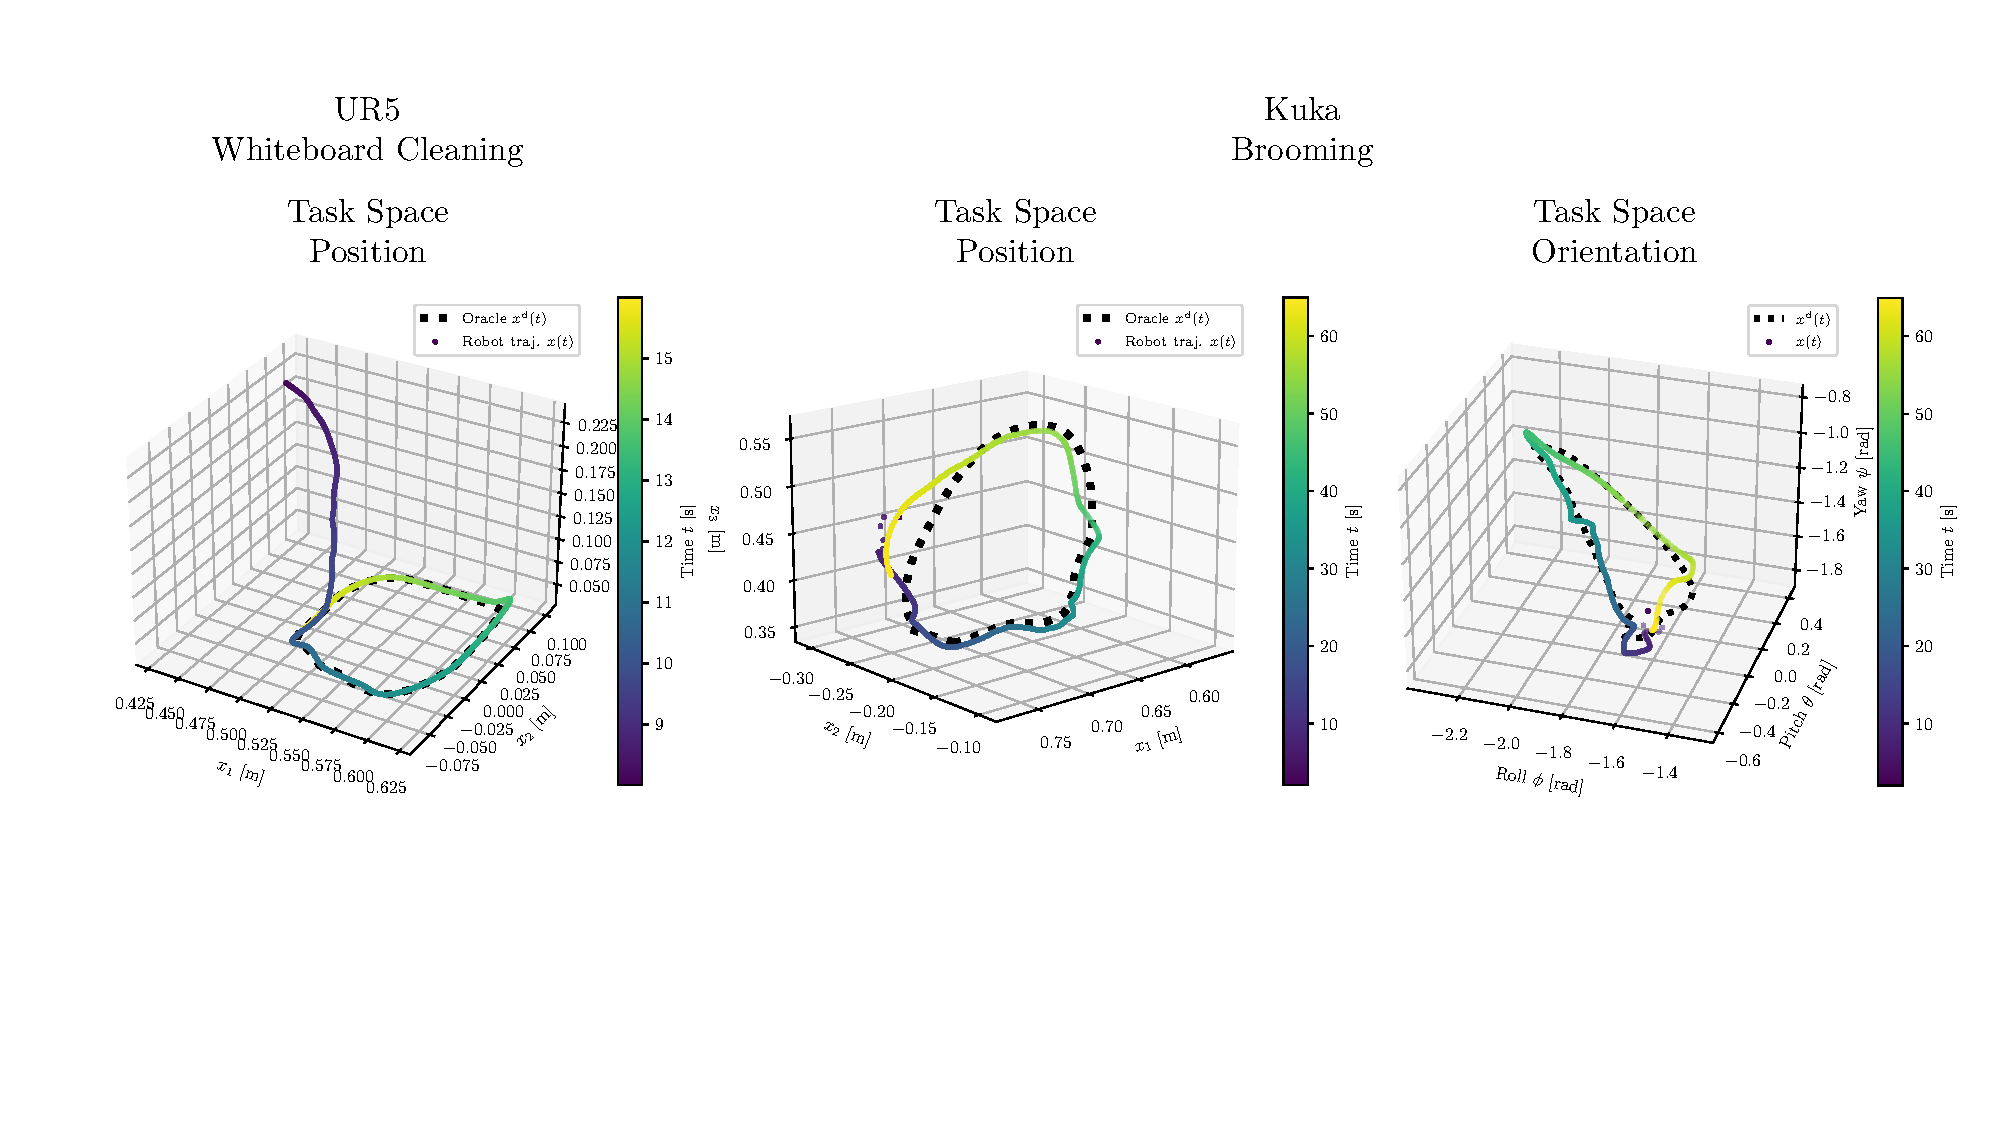
\includegraphics[width=1.0\linewidth]{osmp/figures/kinesthetic_teaching_results/kinesthetic_teaching_results_v1_cropped.pdf}
    \caption{\textbf{Real-world results for learning orbital motion primitives from kinesthetic demonstrations.}
    In the first column, we show the results for a whiteboard cleaning task executed with the UR5 manipulator, and in the second and third columns, we show the results for a booming task executed with the KUKA robot.
    In both cases, the demonstration was provided via kinesthetic teaching, and the \gls{OSMP} was trained on the resulting periodic oracle.
    For the UR5 manipulator, the \gls{OSMP} learns the motion of the end-effector position in three dimensions. For the KUKA manipulator, we learn both the motion of the end-effector position and orientation.
    The color signifies the time when executing the task using the trained \gls{OSMP}.
    }
    \label{fig:osmp:kinesthetic_teaching_results}
\end{figure}

\subsection{Learning Orbital Motion Primitives from Kinesthetic Demonstrations}
% \begin{itemize}
%     \item Demonstrate how our method is able to be applied to demonstrations that were created using kinesthetic teaching and that it is able to accomplish real-world tasks.
%     \item Show results for UR5 whiteboard cleaning and KUKA brooming tasks.
% \end{itemize}

In this section, we examine demonstrations captured through kinesthetic teaching, which tend to be more jerky and less smooth compared to the well-defined geometric oracles discussed earlier. Moreover, when demonstrating periodic motion, the oracle usually does not perfectly close, as a spatial offset remains between the starting and ending poses, which makes it more challenging to fit the limit cycle to the oracle accurately

In Fig.~\ref{fig:osmp:kinesthetic_teaching_results}, we present results for learning \glspl{OSMP} on cleaning tasks that were provided via kinesthetic teaching. Specifically, we consider a whiteboard erasure task on a UR5 manipulator and a brooming task on a KUKA cobot.
While in the case of the UR5, we only encode the spatial translation (i.e., positions) of the end-effector in the \gls{OSMP}, we also consider the motion of the end-effector orientation in the case of the KUKA task. 
In the case of the UR5 robot, we observe a fast convergence onto the limit cycle and, subsequently, good tracking of the oracle with only minor deviations at the point where we fused the start/end points of the periodic motions.
When deploying the \gls{OSMP} on the KUKA \gls{Cobot}, we notice a larger tracking error - likely due to the challenging oracle with $n=6$ \glspl{DOF} and the low feedback gains used in the low-level controller.


\begin{figure}[h]
    \centering
    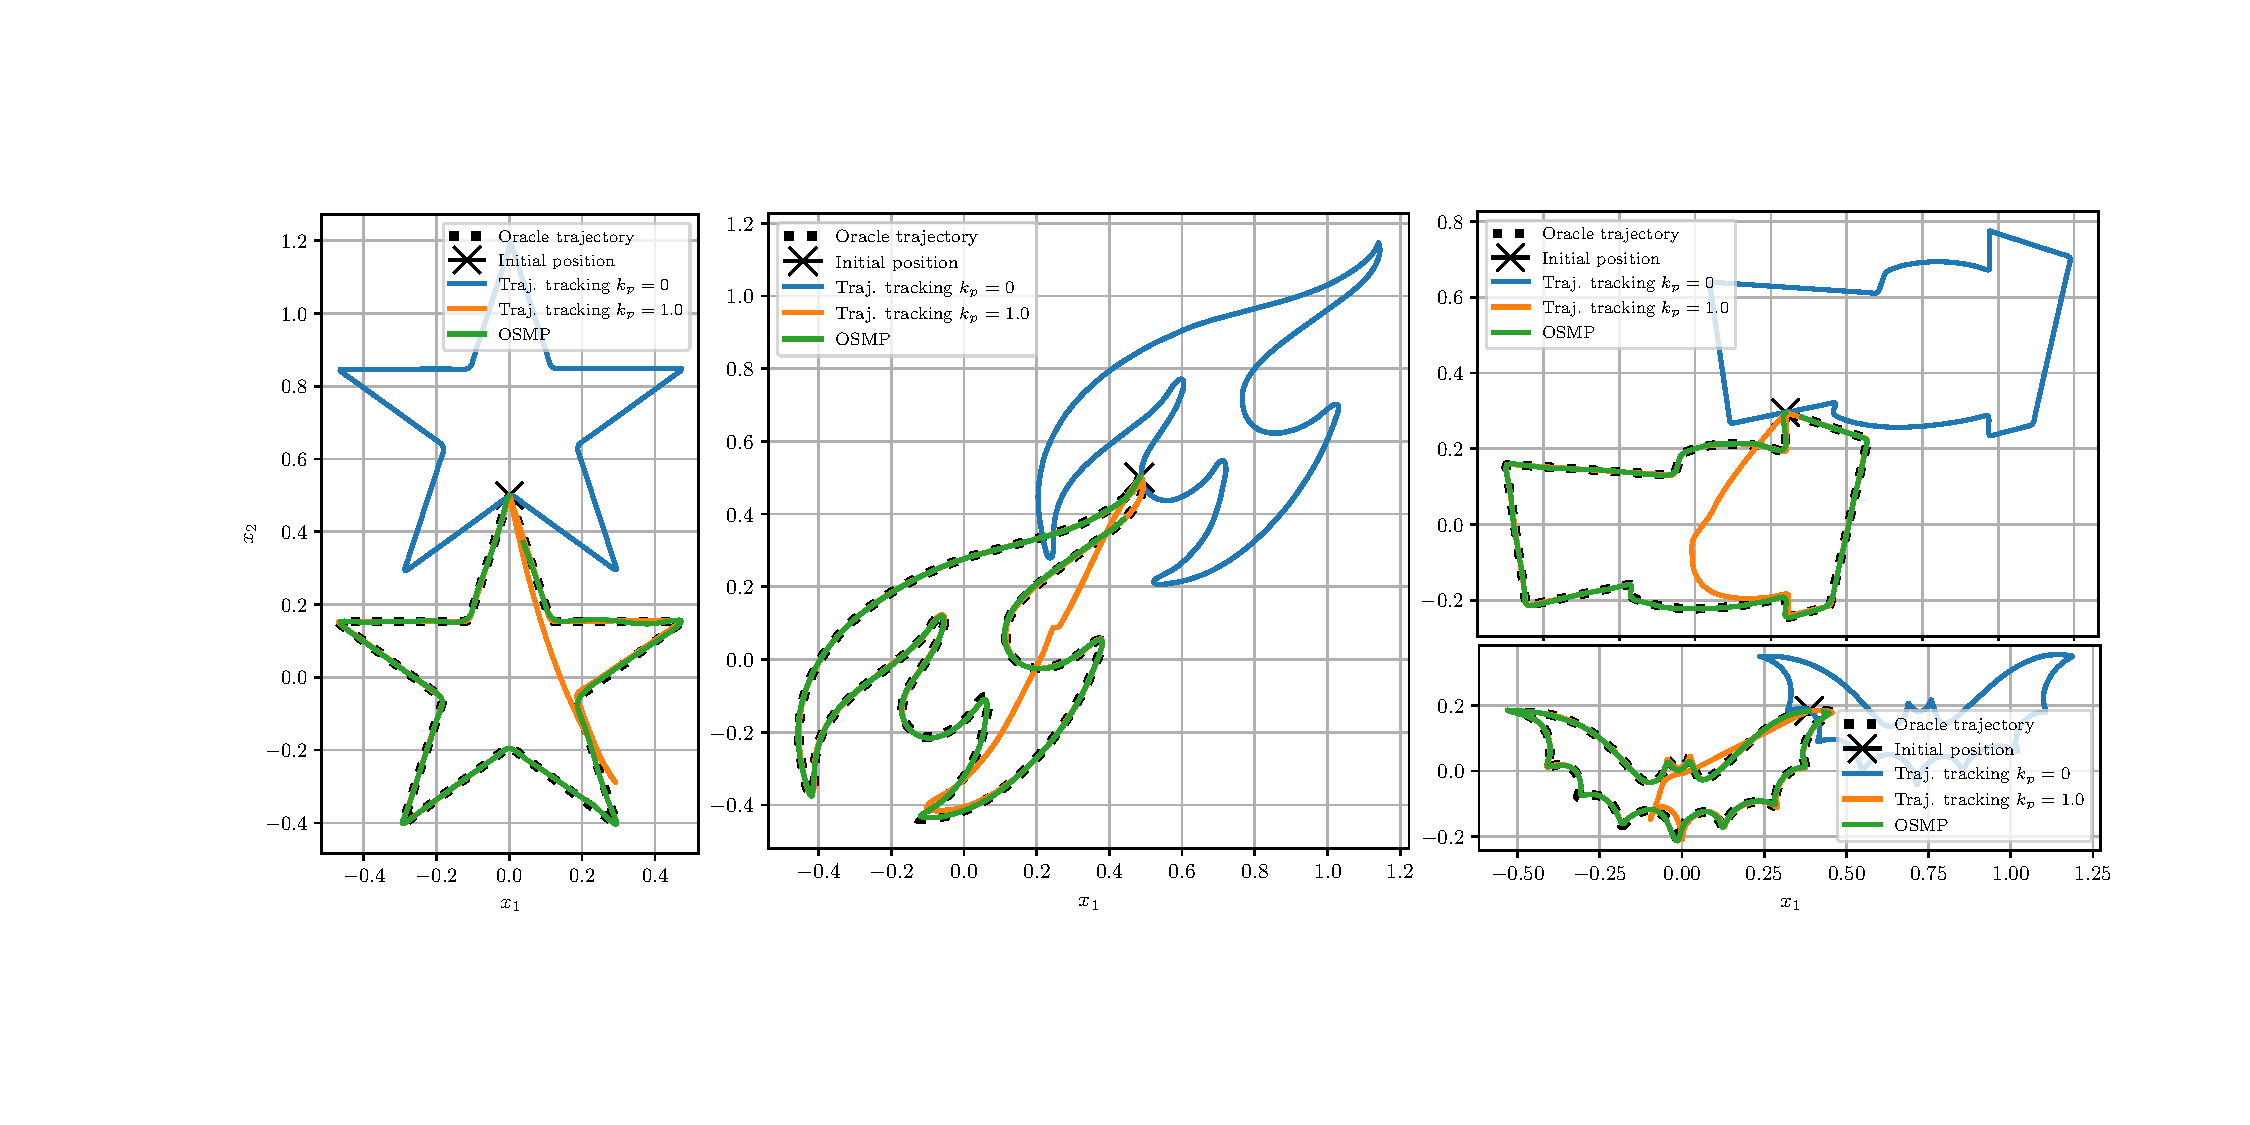
\includegraphics[width=1.0\linewidth]{osmp/figures/compliance_results/compliance_results_v1_cropped.pdf}
    \caption{\textbf{Analyzing the compliance and motion behavior.}
    Simulations with time perturbations where we compare the behavior of traditional, time-parametrized trajectory tracking controllers against the \glspl{OSMP}. Here, the dashed black lines denote the oracles/demonstrations, the solid blue lines the behavior of a pure feedforward trajectory tracking controller $\dot{x}(t) = \dot{x}^\mathrm{d}(t)$ operating on a time-parametrized reference $\dot{x}^\mathrm{d}(t)$, the orange line the behavior of an error-based feedback trajectory tracking controller $\dot{x}(t) = \dot{x}^\mathrm{d}(t) + k_\mathrm{p} \, (x^\mathrm{d}(t) - x(t))$ with $k_\mathrm{p} = 1$, and the green line the behavior of the learned \gls{OSMP}. Compared to nominal scenarios, we perturb the time reference - i.e., the time reference exhibits a $\pi$ offset in phase with respect to the initial position.
    }
    \label{fig:osmp:compliance_results}
\end{figure}

\subsection{The Learned Policies Exhibit Compliant and Natural Motion Behavior}
% \begin{itemize}
%     \item The goal of this subsection is to show how a policy parametrized by a dynamic system is much more compliant and exhibits more natural and predictable motions than a traditional time-parametrized trajectory tracking controller.
%     \item Show a simulated 2D toy case where we perturb the time reference. Then, we compare the trajectories of a) a time-parametrized pure feedforward controller, b) a time-parametrized feedforward+feedback controller, and c) our orbital motion primitive. The feedforward controller would diverge upon time perturbation, the feedforward+feedback controller would be able to track the trajectory but exhibit unnatural motions, and the motion primitives are not affected by a perturbation in the time reference.
%     \item Show the results of the real-world experiments where the dynamical motion primitive exhibited a much more compliant behavior upon physical interaction of the robot than the time-parametrized trajectory tracking controller.
% \end{itemize}

We aim for robots in human-centric environments to demonstrate robust, compliant, and predictable behavior. Specifically, \emph{robustness} means that if a robot deviates from its intended path—perhaps due to a disturbance—it will always converge back to the desired motion. \emph{Compliance} indicates that robots should exert only minimal forces when coming into contact with humans, and \emph{predictability} ensures that their motions are sufficiently consistent for humans to anticipate their behavior and respond appropriately.

In this section, we compare the reaction upon disturbances and perturbations of \glspl{OSMP} against traditional trajectory tracking controllers that rely on a time-parametrized trajectory.
Such error-based feedback controllers are usually given in the form
\begin{equation}\label{eq:osmp:trajectory_tracking_controller}
    \dot{x}(t) = \dot{x}^\mathrm{d}(t) + K_\mathrm{p} \, (x^\mathrm{d}(t) - x(t)),
\end{equation}
where $K_\mathrm{p} \in \mathbb{R}^{n \times n}$ is a proportional feedback gain that operates on the error between the current position $x(t)$ and the desired position $x^\mathrm{d}(t)$. In practice, we choose a scalar $k_\mathrm{p} \in \mathbb{R}_+$ such that $K_\mathrm{p} = k_\mathrm{p} \, \mathbb{I}_{n}$. We stress here the reliance on a time-parametrized trajectory provided in the form $(x^\mathrm{d}(t),\dot{x}^\mathrm{d}(t)) \: \forall \: t \in [t_0, t_\mathrm{f}]$. 
We evaluate in simulation three motion controllers: a pure feedforward trajectory tracking controller, which we gather by setting $k_\mathrm{p} = 0$, and an error-based feedback controller with $k_\mathrm{p} > 0$, and the learned \gls{OSMP}.
In this setting, we are particularly interested in analyzing the behavior of the motion controllers upon encountering an external disturbance that perturbs the state of the system with respect to the time reference. For this, we shift the time reference when initializing the system by half a period (i.e., a phase shift of $\pi$~rad).

The results in Fig.~\ref{fig:osmp:compliance_results} show that the pure feedforward trajectory tracking controller entirely drifts off the desired trajectory. When adding an error-based feedback term, the traditional trajectory tracking controller is able to recover and rejoin the demonstrated trajectory after a bit. However, while doing so, the feedback term generates a very aggressive correction action, which could cause incompliant behavior and would not seem natural to humans. Instead, the \gls{OSMP}, which is solely conditioned on the system state and not time, is not affected by the perturbation of the time reference and perfectly tracks the demonstration while exhibiting compliant and natural behavior.


\subsection{Achieving Phase Synchronization Across Multiple Motion Primitives}
% \begin{itemize}
%     \item Motivate why phase synchronization is important and for which applications it can be useful.
%     \item Showcase a 2D toy example where we are synchronizing three or more learned motion primitives.
%     \item Show the real-world results from the turtle pool tests where i) the turtle doesn't swim when the flippers are not synchronized, ii) how we achieve the flipper synchronization and how that makes the turtle swim.
% \end{itemize}

In many practical applications, such as locomotion, synchronizing multiple motion policies is critical. In this section, we illustrate how our approach can synchronize multiple learned \glspl{OSMP} by evaluating the polar phase of each and then aligning them via an error-based feedback controller~\citep{dorfler2014synchronization}. Crucially, we only adjust the velocity magnitude without altering the system’s spatial motion, thereby preserving the imitation and convergence properties of each learned motion policy.

\begin{figure}[h]
    \centering
    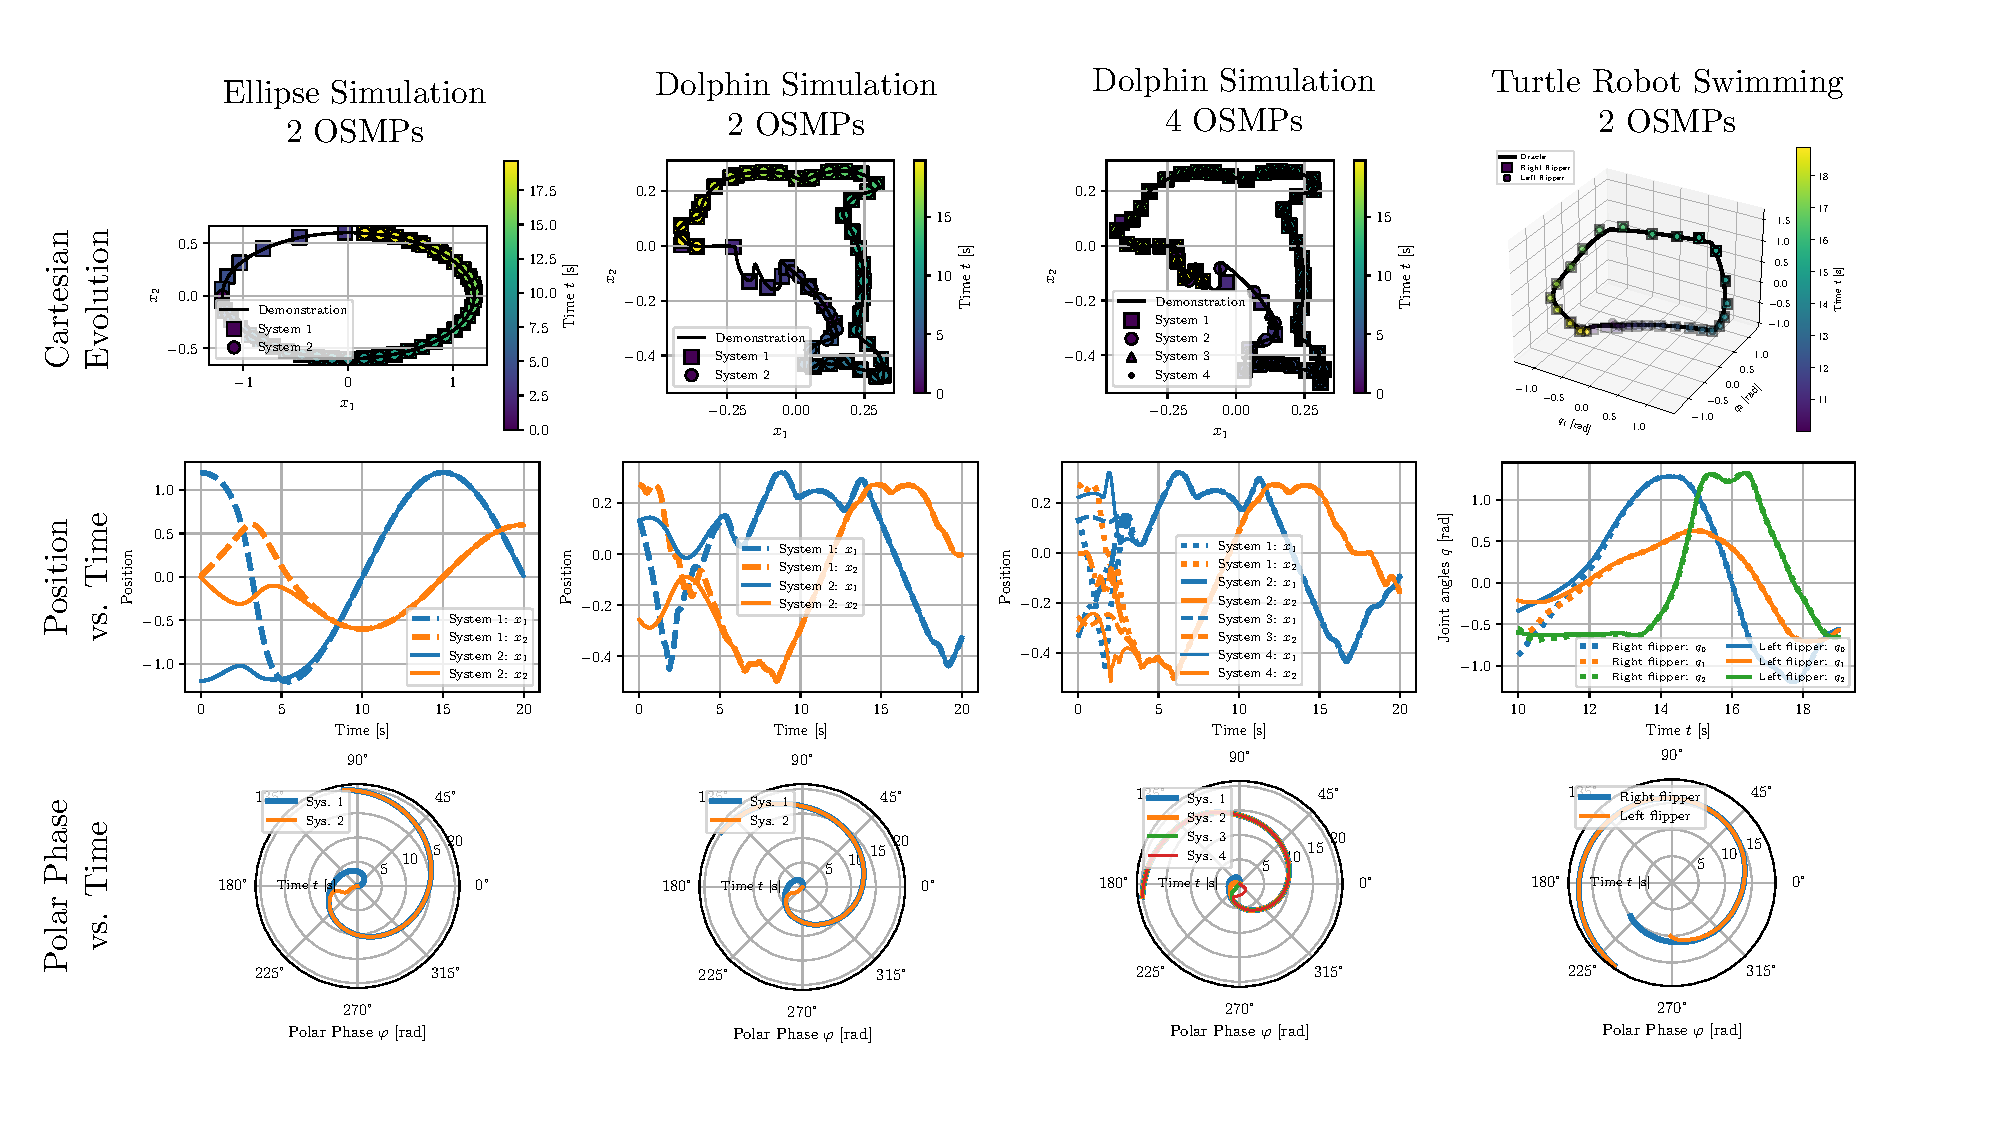
\includegraphics[width=1.0\linewidth]{osmp/figures/phase_sync_results/phase_sync_results_v1_cropped.pdf}
    \caption{\textbf{Phase synchronization of \glspl{OSMP}.}
    Results for the phase synchronization of multiple \gls{OSMP} systems. The first row shows the Cartesian-space evolution of each \gls{OSMP}, where the color of the markers communicates the time information. The second row shows the position vs. time, and the last row shows the polar phase $\varphi$ of the systems over time. 
    The first three columns show simulation results for \glspl{OSMP} trained on ellipse and Dolphin demonstrations, respectively. In all rows, we synchronize the motion of two systems/\glspl{OSMP}, except for the third row, where we synchronize four systems.
    }
    \label{fig:osmp:phase_sync_results}
\end{figure}

In Fig.~\ref{fig:osmp:phase_sync_results}, we show simulation and experimental results for synchronizing two and four \glspl{OSMP}. The outcomes illustrate how the controller identifies the most efficient strategy to align the \glspl{OSMP}, achieving rapid polar phase synchronization. A proportional gain determines the aggressiveness of the synchronization process. The simulation results confirm that the phase synchronization approach is effective not only for two systems but also for four or more.

Regarding experimental findings, we examined the swimming performance of the Crush turtle robot. Tests in a swimming pool revealed that the robot can swim effectively only when both front flippers—the primary means of locomotion in water~\citep{van2022new, van2023soft}—are fully synchronized. In practice, even aside from external disturbances and inherent differences between the flippers, desynchronization occurs already during initialization when the flipper arms start in slightly different configurations with varying polar phases. Our results show that using our method, the two flipper arms synchronize in less than a quarter of a period, thereby enabling the turtle robot to swim effectively.

\subsection{Smooth Interpolation Between Motion Behaviors via Encoder Conditioning}
% \begin{itemize}
%     \item Motivate how encoder conditioning enables the incorporation of multiple oracles in the same motion primitive.
%     \item Motivate why we would (ideally) want to achieve smooth interpolation between oracles.
%     \item Showcase 2D toy examples for the interpolation between two or more oracles. We also show that this works in the real world on the UR5 robot.
%     \item Demonstrate how we can learn both forward and reverse turtle swimming with the same motion primitive using encoder conditioning and how we can smoothly interpolate between the two motions.
% \end{itemize}

As we move toward generalist motion policies~\citep{o2024open, black2024pi0, gemini2025robotics}, the motion policy must integrate not just a single behavior but a range of diverse behaviors conditioned on the task, the robot’s state, and its perception of the environment. In particular, we aim to leverage in the future semantic encodings from sources like \glspl{VLM} as motion conditioning. However, this aspect has not been sufficiently explored within the realm of dynamic motion primitives. Moreover, there may be many scenarios where interpolating between two or more motion behaviors from the training set is beneficial, which is not supported by the current methods~\citep{rana2020euclideanizing, perez2023stable, perez2024puma, sochopoulos2024learning, zhi2024teaching}.
%
One example involves different surface cleaning motions, where the specific cleaning action is selected based on the surface material. In this case, the robot should be able to transition smoothly between cleaning motions when moving from one surface to another. Another example is locomotion: if oracles are available for walking on flat terrain and for stepping over steep stairs, then for obstacles or moderately steep, stair-like terrain, it may be beneficial to interpolate between these two oracles, while we would want to preserve the naturalness of the motion.

\begin{figure}[h]
    \centering
    \includegraphics[width=1.0\linewidth]{osmp/figures/conditioning_results/conditioning_results_v1_cropped.pdf}
    \caption{
    \textbf{Smooth interpolation between distinct motion behaviors via encoder conditioning.}
    Results demonstrating the conditioning of the encoder on multiple learned motion behaviors, including smooth interpolation between behaviors.
    The first row shows the behavior of an OSMP that was trained jointly on a horizontal ellipse ($z=0$) and a vertical ellipse ($z=1$).
    The second row shows the behavior of an OSMP that was trained jointly on a horizontal ellipse ($z=0$) and a square ($z=1$).
    The third row shows the behavior of an OSMP that was trained jointly on a square ($z=0$) and the MIT CSAIL logo ($z=1$).
    The first four columns present the simulated behavior for a constant conditioning $z$ between $z=0$ and $z=1$, where the black dashed line denotes the two oracles used for training and the green line the simulated trajectory that is a function of the velocity field for the given conditioning $z$.
    The fifth column contains a simulation where the conditioning is slowly increased, where the color indicates the conditioning $z$.
    Similarly, the sixth column includes real-world results obtained with a UR5 manipulator where the conditioning is slowly increased from $z=0$ at $t=0$ to $z=1$ at $t=140$~s. Here, the color indicates the time.
    }
    \label{fig:osmp:conditioning_results}
\end{figure}

In this work, we introduce task conditioning for the bijective encoder using a conditioning variable $z \in \mathbb{R}$. This variable enables us to select the desired motion behavior online by providing the appropriate $z$ value. Moreover, we train the \gls{OSMP} so that the learned motion policy smoothly interpolates between two or more motion behavior conditionings (e.g., $z=0$ and $z=1$). As shown in Fig.~\ref{fig:osmp:conditioning_results}, our simulations and real-world experiments with a UR5 manipulator demonstrate that (a) the same \gls{OSMP} can accurately learn multiple motion behaviors and (b) smooth interpolation between these behaviors is achievable by adjusting the conditioning. Importantly, switching between motion behaviors does not require an elaborate sequence; once a new $z$ is set, the \gls{OSMP}’s convergence guarantees ensure that the system quickly adapts to the new behavior.
\section{Conclusion}
% In this chapter, we presented an approach for learning periodic/cyclical motion from demonstration using \glspl{OSMP}, where the motion policy is, analog to \glspl{DMP}~\cite{ijspeert2002learning, ijspeert2013dynamical}, parametrized by a dynamical system.
% Specifically, we combined the strengths of \gls{ML} approaches, such as expressiveness and the lack of requirements for heuristics, with nonlinear system theory to guarantee that the periodic is tracked via a limit cycle behavior that exhibits orbital stability.
% We achieve this by combining a learned bijective encoder based on Euclideanizing flows~\citep{dinh2016density, rana2020euclideanizing} that establishes a diffeomorphism between the oracle and the latent space and inspectable and fixed dynamics in latent space given by supercritical Hopf birfurcation~~\cite{strogatz2018nonlinear}.
% Compared to existing work~\cite{zhi2024teaching}, we significantly improve the accuracy of the matching between periodic demonstration and the generated limit cycle.
% Additionally, we benchmark the \glspl{OSMP} against standard \gls{ML} methods which reveals that they guarnatee convergence while standard \gls{ML} methods such as \glspl{MLP} or \glspl{RNN} often exhibit spurious attractors.
% Also, we extensively validate the proposed method in the real-world on various robot embodiments, including robotic manipulators and \glspl{Cobot}, soft robots, and bioinspired hybrid soft-rigid underwater robots.
In this chapter, we introduced an approach for learning periodic/cyclical motions from demonstrations using \glspl{OSMP}, where—similar to \glspl{DMP}~\citep{ijspeert2002learning, ijspeert2013dynamical}—the motion policy is parametrized by a dynamical system. We combined the advantages of \gls{ML} methods, such as their high expressiveness, with nonlinear system theory to ensure that the periodic motion is tracked via a limit cycle that exhibits \glsxtrfull{OS}. This is achieved by integrating a learned bijective encoder based on Euclideanizing flows~\citep{dinh2016density, rana2020euclideanizing}, which establishes a diffeomorphism between the oracle and latent space, with fixed, inspectable dynamics in latent space provided by a supercritical Hopf bifurcation~\citep{strogatz2018nonlinear}. Compared to previous work~\citep{zhi2024teaching}, our approach significantly improves the accuracy of matching the periodic demonstration to the generated limit cycle. Furthermore, benchmarking against standard \gls{ML} techniques shows that \glspl{OSMP} guarantee convergence, whereas traditional methods such as \glspl{RNN} and \glspl{NODE}~\citep{zhi2024teaching} often exhibit spurious attractors. We also validate our method extensively in real-world settings across various robotic platforms, including robotic manipulators and \glspl{Cobot}, soft robots, and bioinspired hybrid soft-rigid underwater robots.

% Moreover, we devise several techniques that increase the capability of dynamic motion primitives, including online reshaping of the velocity field that adjust the convergence characteristics as needed without requiring retraining, the synchronization of multiple \glspl{OSMP} in their phase by leveraging a error-based feedback term, and the capability to learn several distinct motion behaviors with the same motion policy by conditioning the encoder on the task/motion behavior. After adding a loss term, we are even able to smoothly interpolate between two motion behaviors. 
Moreover, we developed several techniques to enhance the capabilities of dynamic motion primitives. These include online reshaping of the velocity field to adjust convergence characteristics without retraining, synchronizing multiple \glspl{OSMP} in phase via an error-based feedback term, and enabling the same motion policy to learn multiple distinct behaviors by conditioning the encoder on the task. With the addition of a tailored loss term, we can even achieve smooth interpolation between two motion behaviors.

% For future work, it would be interesting to allow the same motion primitive to exhibit multiple classes of attractors~\citep{strogatz2018nonlinear}, including \gls{GAS} (for point-to-point motions), \gls{MS} (for multiple goals with equal value), and \gls{OS} (for periodic motions).
% A first step would be to build on top of the formulation employed in this paper, as the supercritical Hopf bifurcation can capture both exhibit a single, isolated equilibrium and limit cycle behavior if we were to add an additional parameter that would allow us to control that~\citep{strogatz2018nonlinear}.
% Furthermore, it seems timely and obvious, to condition the encoder on the outputs/embeddings of modern \glspl{VLM}~\citep{o2024open, touvron2023llama, grattafiori2024llama}, which would allow to significantly increase the generalization, reasoning, and planning capabilities of the motion policies while preserving the insight, robustness, compliance, and convergence guarantees that \glspl{DMP} exhibit.
For future work, it would be intriguing to enable a single motion primitive to exhibit multiple classes of attractors~\citep{strogatz2018nonlinear}, such as \gls{GAS} for point-to-point motions, \gls{MS} for multiple equally valued goals, and \gls{OS} for periodic motions. An initial step could build on the formulation presented here, as the supercritical Hopf bifurcation can capture both a single isolated equilibrium and limit cycle behavior if an additional \emph{attractor type} parameter is introduced. Furthermore, it appears timely to condition the encoder on the outputs or embeddings of modern \glspl{VLM}~\citep{o2024open, touvron2023llama, grattafiori2024llama}, which would significantly enhance the generalization, reasoning, and planning capabilities of the motion policies while preserving the insight, robustness, compliance, and convergence guarantees inherent to \glspl{DMP}.
